\documentclass[12pt]{article}
\usepackage[utf8]{inputenc}
\usepackage[spanish]{babel}

\usepackage{amsmath}
\usepackage{amsfonts}
\usepackage{graphicx}
\usepackage{xcolor}
\usepackage{subfigure}
\usepackage{hyperref}
\usepackage{tikz}
\usepackage{cleveref}
\usepackage{microtype}
\usepackage{geometry}
\usetikzlibrary{calc}
\usetikzlibrary{circuits}
\renewcommand{\arraystretch}{1.5}
\renewcommand{\baselinestretch}{1.5}
\title{TFG}
\author{Francisco Gómez Prieto}
\usepackage{amssymb}
\usepackage{theorem}
\usepackage{color}
\usepackage{amscd}
%\usepackage{showidx}
\usepackage{textcomp}
\usepackage{pdfpages}
\usepackage{afterpage}
\usepackage{makeidx}
\usepackage{graphicx}
\usepackage{caption}
\usepackage{float}
\usepackage{wrapfig}
\usepackage{listings}
\usepackage{multicol}
\usepackage{cite}


%PARA ESCRIBIR EL SÍMBOLO DEL EURO.
%\def\eu{\,\hbox{\raise .36em\hbox to0pt{\vrule height0.5pt%
%width.55em depth0pt\hss}%
%\raise .25em\hbox to0pt{\vrule height0.5pt width.5em%
%depth0pt\hss}\hskip.02em\sf C}\,}

% Imprime la fecha de revisión y la etiqueta
% 'Draft Version' (From Josullvn, CS, CMU)
%%%%%%%%%%%%%%%%%%%%%%%%%%%%%%%%%%%%%%%%%%%%
%\newcommand{\reviewtimetoday}[2]{\special{
%!userdict begin /bop-hook{gsave 20 710
%translate 45 rotate 0.8 setgray
%/Times-Roman findfont 12 scalefont setfont
%0 0 moveto (#1) show 0 -12 moveto (#2) show grestore}def end}}
%\reviewtimetoday{\today}{Draft Version}

\setlength{\textheight}{21cm} \setlength{\topmargin}{-.5cm}
\setlength{\footskip}{2cm}
\setlength{\oddsidemargin}{1.5cm}
\setlength{\evensidemargin}{-0.25cm}
\setlength{\textwidth}{15cm}

%\usepackage{fancyhdr}
%\pagestyle{fancy}
%\fancyhf{}
%\fancyhead[RE]{\MakeUppercase{CAP.\, \thechapter}}
%\fancyhead[LO]{}
%\fancyhead[RO,LE]{\bfseries \thepage}
%\fancyhead[CE]{\leftmark}
%\fancyhead[CO]{\rightmark}

%\renewcommand{\chaptermark}[1]{\markboth{\MakeUppercase{#1}}{}}
%\renewcommand{\chaptermark}[1]{\markboth{\chaptername\, \thechapter. #1}{}}
\renewcommand{\sectionmark}[1]{\markright{\thesection. #1}}
%\renewcommand{\headrulewidth}{.6pt}
%\renewcommand{\headrule}{\setlength=15cm}

\setlength{\headheight}{2.5\headheight}
%\renewcommand{\headrule}{\leftskip=.5cm}
%\fancyfoot{}
%\renewcommand{\headrule}{\vbox to 0pt{\hbox to 50pt}}
%\renewcommand{\headrule}{%
%\makebox[0pt][0]{\rule[3\baselineskip]{\linewidth}{0.8pt}}%
%\color[named]{Red}%
%\rule[-.3\baselineskip]{\linewidth}{0.4pt}}

% Limpia el encabezado en las páginas impares vacías
\makeatletter \def\cleardoublepage{
\clearpage\if@twoside \ifodd\c@page\else%
\hbox{}%
\thispagestyle{empty}% Aquí elimina el estilo del encabezado
\newpage%
\if@twocolumn\hbox{}\newpage\fi\fi\fi} \makeatother

\providecommand{\norm}[1]{\lVert#1\rVert}

%\usepackage[active]{srcltx}


\def\blacksquare{\hbox{\vrule width 4pt height 4pt depth 0pt}}
\def\qed{\ \ \ \hbox{}\nolinebreak\hfill $\blacksquare \  \  \  \  $ \par{}\medskip}


\newtheorem{theorem}{Teorema}[section]
\newtheorem{teorema}[theorem]{Teorema}
\newtheorem{lemma}[theorem]{Lema}
\newtheorem{proposicion}[theorem]{Proposición}
\newtheorem{corolario}[theorem]{Corolario}




\newtheorem{ejemplo}[theorem]{Ejemplo}
\newtheorem{definicion}[theorem]{Definición}
\newtheorem{ejercicio}[theorem]{Ejercicio}
\newtheorem{notacion}[theorem]{Notación}


\newtheorem{observacion}[theorem]{Observación}

\numberwithin{equation}{section}


\newcommand{\teor}{\begin{teorema}}
\newcommand{\eteor}{\end{teorema}}
\newcommand{\prop}{\begin{proposicion}}
\newcommand{\eprop}{\end{proposicion}}
\newcommand{\coro}{\begin{corolario}}
\newcommand{\ecoro}{\end{corolario}}
\newcommand{\lema}{\begin{lemma}}
\newcommand{\elema}{\end{lemma}}
\newcommand{\ejer}{\begin{ejercicio}}
\newcommand{\eejer}{\end{ejercicio}}
\newcommand{\obse}{\begin{observacion}}
\newcommand{\eobse}{\end{observacion}}
\newcommand{\defi}{\begin{definicion}}
\newcommand{\edefi}{\end{definicion}}
\newcommand{\demo}{\begin{proof}[Demostración]}
\newcommand{\edemo}{\end{proof}}
\newcommand{\ejem}{\begin{ejemplo}}
\newcommand{\eejem}{\end{ejemplo}}
\newcommand{\nota}{\begin{notacion}}
\newcommand{\enota}{\end{notacion}}
\newcommand{\nada}{\begin{naida}}
\newcommand{\enada}{\end{naida}}
\newcommand{\vaci}{\begin{vacio}}
\newcommand{\evaci}{\end{vacio}}
\newcommand{\sucesion}{(x_n)_{n\in \mathbb{N}}}
\newcommand{\sucesionpelada}{(x_n)}
\usepackage[all]{xypic}

%\newenvironment{flushenum}{  %%% NO INDENTA LOS ITEMS EN UNA ENUMERACIÓN
%\begin{enumerate}            %%%
%  \setlength{\leftmargin}{0pt}%%%
%}{\end{enumerate}}            %%%



\usepackage{enumitem}  
%PERMITE, POR EJEMPLO, QUITAR "INDENTS" DE LOS "ITEMS" (Poniendo %%%%%%%%%%%%%%%%%%%%%%%%\begin{enumerate}[leftmargin=*] %+y, luego, todo igual %que siempre.)

%\includegraphics




\usepackage[final]{epsfig}
\date{}
\makeindex

\begin{document}
\pagestyle{empty}
\lstset{language=Java}
\includepdf[pages={8}]{normativa3.pdf}

\newpage
~

\newpage
Fernando Javier Álvarez Franco, profesor del departamento de Ingeniería Eléctrica, Electrónica y Automática de la universidad de Extremadura.

INFORMA:

Que D. Francisco Gómez Prieto ha realizado bajo su dirección el Trabajo de Fin de Grado. Considera que la memoria reune los requisitos necesarios para su evaluación.

\medskip

\begin{flushright}
Badajoz, 26 de Junio de 2019
\end{flushright}

\vspace{8\baselineskip}
\begin{center}
Fdo. Fernando Javier Álvarez Franco.
\end{center}
\newpage
~
\newpage

Agradecimientos. TO-DO

\newpage
~
\newpage
\setcounter{page}{1}
\pagestyle{plain}
\tableofcontents

\newpage
~

\newpage
\section*{Resumen}
\addcontentsline{toc}{section}{Resumen}
El objetivo de este trabajo de fin de grado es estudiar donde se encuentra la tecnología de identificación de patrones motores y realizar una aplicación práctica sobre la detección del tipo de movimiento centrándonos en cuatro tipos: Estacionario, corriendo, andando y caída.

Con este objetivo presente, se utilizaran los medios más actualizados para la realización del proyecto experimental, siendo, como se verá más adelante, las redes neuronales o diversas técnicas de inteligencia artificial lo más avanzado. 

Además, se usará un smartwatch para realizar la toma de datos, permitiendo así tomar datos muy precisos sin agotar la batería del smartphone del usuario. Otro objetivo es el tener una interfaz sencilla e intuitiva, para que personas adultas o ancianas no tengan ningún tipo de problema al utilizar el sistema.


\newpage
\section*{Abstract}
\addcontentsline{toc}{section}{Abstract}


The objective of this work is study about the technology involving vital signal and create an app about movement patterns involving these 4 types of movements: Stationary, running, walking and falling down.

With that objective in mind, we will use the most advanced methods to do the experimental project, and neural networks and other algorithms of artificial intelligence are those advanced methods.

Also, we will use a smartwatch as data retriever. This way we will obtain very precise data without draining the user's smartphone battery. Another objective is having a simple and intuitive interface, so the elderly and adults alike don't have any problem using the system.

\newpage
\section{Introducción}

En este trabajo se pretende clasificar los tipos de movimientos mediante un dispositivo wearable Android. Para ello se van a usar un smartphone Android, un reloj con sistema operativo wearOS, que es simplemente Android Wear actualizado.

Para la clasificación se va a usar un sistema de inteligencia artificial, basado en redes neuronales cuyo objetivo es ir identificando en tiempo real el tipo de movimiento y mostrar los resultados de esta clasificación en pantalla.

Este tipo de monitorización contínua es muy interesante ya que hay enfermedades en las que un estudio con seguimiento continuo puede ser usado para establecer el estado de la enfermedad en el usuario y a partir de esta información mejorar la calidad de vida de los pacientes.

Otra aplicación más comercial sería la detección de distintos tipos de ejercicio para una optimización del movimiento realizado por atletas profesionales o para amateurs, una simple aplicación de ejercicio para contar kilocalorias, que es una opción bastante demandada si nos fijamos en el número de Apps que hay en las stores de Android y iOS.

La principal contribución de este trabajo es la implementación en WearOS, permitiendo su uso en multitud de dispositivos y tomando datos mucho más útiles que si los tomara desde el smartphone, ya que el reloj es un dispositivo situado en la muñeca, al contrario que los smartphones. Esto es una ventaja pues permite ahorrar el trabajo de situar el dispositivo con respecto al cuerpo, pues está fijo, simplificando el código de forma considerable.
\section{Antecedentes}
A continuación se hará un recorrido ordenando los momentos clave que ponen en contexto el trabajo aquí realizado. Para ello, se va a hacer un recorrido histórico mencionando los momentos claves para la tecnología usada, empezando por las redes neuronales y posteriormente los acelerómetros y los algoritmos de clasificación de movimiento.
\subsection{Redes neuronales e Inteligencia artificial.}
A lo largo de la historia de la humanidad, está ha soñado con crear máquinas que tuvieran inteligencia. Como todo, ya en la antigua Grecia se había mencionado el tema, con las leyendas de Hefesto, que creó varios autómatas para que le ayudaran en sus trabajos de herrería. Por  desgracia, aquella habilidad quedaba limitada a dioses por aquel entonces.

A lo largo de los siglos, se fue nutriendo esta rama de la ciencia, pero se puede decir que hasta mediados del siglo XX no hubo avances reales.

Las redes neuronales es un campo multidisciplinar en el que han trabajado informáticos, biólogos, médicos, físicos y matemáticos por nombrar solo algunos. Al ser una tecnología basada(vagamente) en la biología humana, en la estructura de nuestro cerebro, es imposible que hubiera habido un desarrollo previo a los descubrimientos de nuestro compatriota Santiago Ramón y Cajal.

\subsubsection{Primera ola(1949-1969)}

Se podría decir que la primera ola de investigación rigurosa en el campo comenzó cuando D.O. Hebb publicó su libro,\textit{The organization of behavior}, donde se propone la primera ley de aprendizaje, que sirvió como base para el entrenamiento de las primeras redes neuronales.

Durante esta época, se desarrollaron las primeras redes neuronales que resolvían problemas simples, inicialmente en circuitos electrónicos y posteriormente en simulaciones por ordenador, mucho más flexibles.

Estos resultados positivos hicieron que en el campo hubiera mucha investigación, y se produjeran grandes avances, como el algoritmo del Perceptron, en 1957\cite{rosenblatt1957perceptron}. Este algoritmo aún hoy en día es la base del campo y sigue siendo un algoritmo útil, con pequeñas mejoras.

Durante esta época, había grandes esperanzas en el campo, aunque solo pudieran resolver los problemas más sencillos. Sin embargo, en 1969 Marvin Minsky publicó su libro, \textit{Perceptrons}\cite{minsky}. En él, con una rigurosa base matemática se exponen los límites a los que se enfrenta los algoritmos de la época y se enumeran diversos problemas sencillos que no pueden resolver las redes neuronales, como por ejemplo una simple puerta XOR. Minsky era un científico respetado y con prestigio, y la publicación de su libro hizo que la investigación y financiación del campo se redujera durante años.
\subsubsection{Segunda ola(1986-1995)}
Durante las dos olas de investigación, las publicaciones no fueron en revistas de prestigio científico, lo cual hizo que la información, además de reducirse, se esparciese, lo que provocó que el trabajo muchas veces no llegara entre investigadores del mismo campo.

Sin embargo, durante las dos olas, no se abandono el trabajo, y debido a las limitaciones de potencia, se centró en dar una base teórica más rigurosa que la anterior.

Sin embargo, en 1986 se publicó el algoritmo de retropropagación\cite{Rumelhart:1988:LRB:65669.104451}. Este algoritmo permitía el entrenamiento de múltiples capas en un perceptrón, permitiendo la resolución de problemas que el Perceptron original no podía resolver, que habían sido recopilados por Minsky en su libro. Este algoritmo, aunque publicado en 1986 por Rumelhart \textit{et al}, ya había sido descubierto y aplicado antes, pero como se comentó en los párrafos anteriores, la investigación estaba muy desperdigada en diversas revistas y no siempre llegaba a todos. Cabe mencionar en especial a Paul Werbos, que en 1974 en su tesis ya se aplicaba a redes neuronales\cite{werbos}. 

Esto hizo que en el campo volviera a haber investigación, solo en 1987 hubo cuatro congresos mundiales sobre el tema y más de 500 \textit{papers} sobre el tema.

Por otro lado, en Japón, se desarrolla el Cognitron y el Neocognitron. Estas redes están diseñadas tomando como objetivo la reproducción del funcionamiento de la vista en seres vivos, que con suma facilidad es capaz de reconocer miles de objetos y caras. Estos algoritmos no fueron muy usados en esta época, pues la simpleza del Perceptron multicapa hacía que fuera mucho más usado. Sin embargo, con el paso de los años esta rama fue la base de las redes convolucionales, que son las más utilizadas hoy en día, o mejor dicho, las que dieron lugar a la tercera ola de investigación.

Esta ola acabó a mediados de los 90, debido a varios factores. Primero, llevados por la emoción del momento, los investigadores sobreestimaron las capacidades de la tecnología, y cuando los objetivos que habían ofrecido a los inversores no se cumplieron, bajo la financiación del campo. Por otro lado, otras tecnologías de aprendizaje ofrecieron soluciones a problemas de la época. Esto hizo que la inversión fuera para otras tecnologías.

\subsubsection{Tercera ola(2007-?)}
Se podría decir que esta época fue un resurgimiento de la anterior pero con mucha mas potencia de cálculo.  Esto se debe a varios factores, el primero, el descubrimiento de algoritmos que reducían el tiempo de cálculo en gran medida\cite{doi:10.1162/neco.2006.18.7.1527}. Este algoritmo era fácil de extender a otras aplicaciones, por lo que se redujo mucho el tiempo de cálculo en esta tecnología.

Por otro lado aumenta el número de datos de entrenamiento que se pueden usar para el entrenamiento sin aumento de tiempo de cálculo apenas.

Además, se empieza a aprovechar el hardware mejor. Las tarjetas gráficas se empiezan a usar para hacer los cálculos de entrenamiento de estas redes neuronales, reduciendo aún mas los tiempos de entrenamiento, ya que las tarjetas gráficas tienen una arquitectura  ideal para realización de tareas matemáticas paralelas.

Finalmente, pero no menos importante, esta tercera ola presenta muy buenos resultados, ganando concursos de clasificación. Por ejemplo, el ImageNet Large Scale Visual Recognition Challenge, que paso de un 26.1\% de error a un 15.3\%\cite{concursos} mediante una red neuronal convolucional en un año. Desde ese entonces, todo este tipo de concursos es ganado consistentemente por una CNN(\textit{Convoluted neural network}), actualmente, el error está en torno al 3.0\%.

\subsubsection{Presente(2019)}

Actualmente, el deep learning sigue siendo popular. Por ejemplo nos podemos guiar por un parámetro como las busuqedas de google en los ultimos años.

\begin{figure}[h]
    \centering
    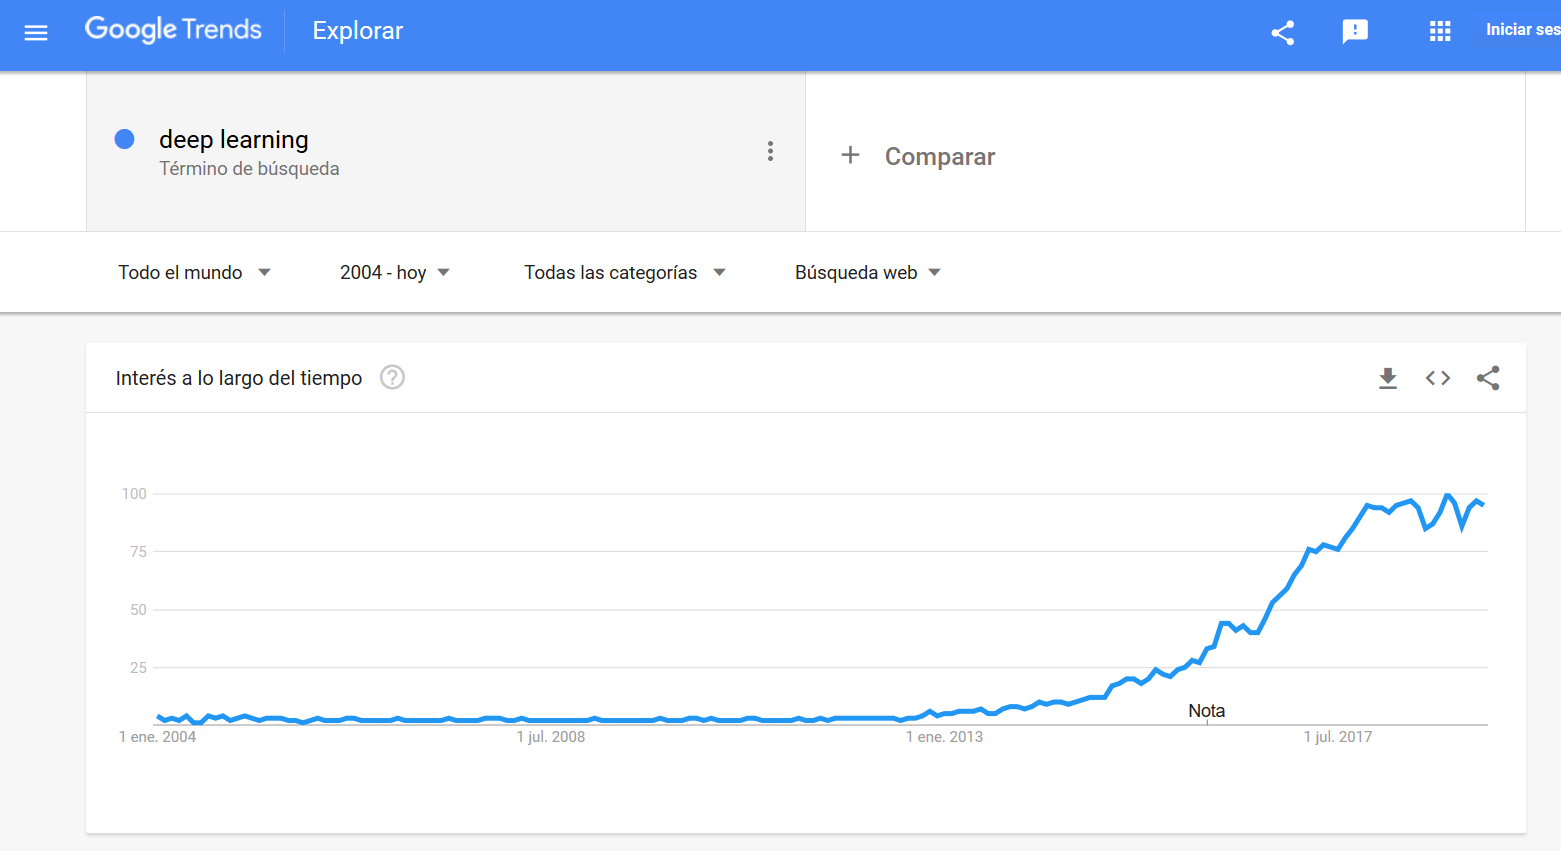
\includegraphics[width=1\textwidth]{growth.png}
    \caption{Busuqedas en google del termino Deep learning}
    \label{fig:growth}
\end{figure}

Se puede tener en cuenta los resultados del LSVRC, en el que en los últimos años ya se supera al ser humano\cite{DBLP:journals/corr/YangH15}, como se puede observar en \ref{fig:errorLSVRC}:

\begin{figure}[h]
    \centering
    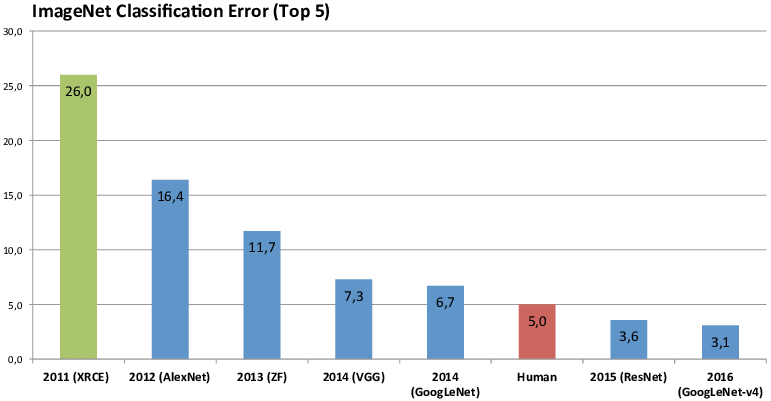
\includegraphics[width=1\textwidth]{Winner-results-of-the-ImageNet-large-scale-visual-recognition-challenge-LSVRC-of-the.png}
    \caption{Error de los ganadores de los años 2011-2016}
    \label{fig:errorLSVRC}
\end{figure}

Estos resultados prometedores y su utilización en problemas del mundo real ha hecho que no haya signos de ralentización en el campo y que hoy en día siga siendo interesante para investigar y trabajar, tanto en el ambito público como en el mercado privado.


\subsubsection{Conclusiones}

Este campo ha sido uno de los más importantes del siglo pasado, pero ha tenido problemas en la investigación y varios parones, entre otras cosas por la falta de potencia de cada época. Además, al ser un campo multidisciplinar hizo que publicara de forma desperdigada en muchas revistas, lo cual hacía que el seguimiento por parte de la comunidad científica fuera difícil. No solo eso, sino que ha cambiado de nombres múltiples veces. Básicamente, es lo mismo hablar de \textit{cybernetics}, redes neuronales artificiales, redes neuronales, \textit{conectionism}, y el más moderno, \textit{deep learning}.

\subsection{Acelerómetros}

Un acelerómetro es un dispositivo que mide la aceleración propia de un cuerpo. Esto quiere decir que en reposo, miden la aceleración de la fuerza de la gravedad en el eje de la tierra, normalmente z.

Su invención fue en 1784, por George Atwood. Se lo conocía como máquina de Atwood, y durante un siglo su utilidad era reducida a estudios científicos. Posteriormente, la industria del automóvil, en busqueda de mayor eficiencia empieza a usarlos en sus vehículos para mejorarla.

\begin{figure}[h]
    \centering
    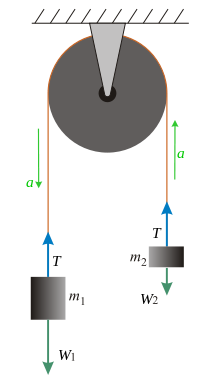
\includegraphics[scale=0.5]{atwood.png}
    \caption{Máquina de Atwood}
    \label{fig:atwood}
\end{figure}

Las necesidades de las industrias emergentes en el siglo XX, como la automovilistica o la minería hicieron que hubiera un gran desarrollo a lo largo del siglo pasado.

\subsubsection{Primera era: 1923-1936}

El primer gran avance en el campo fue en 1923 cuando McCollun y Peters\cite{6534032} desarrollaron el primer acelerometro moderno mediante un sistema de resistencias variables. Consistía en un sistema en forma de E que contenía entre 20 y 55 discos de carbono con un circuito de puente de Wheatstone que conectaba los dos extremos. El circuito puente de Wheatstone se puede ver en la figura \ref{fig:wheatstone}, y sirve para medir resistencias desconocidas entre los dos extremos.

\begin{figure}[h]
    \centering
    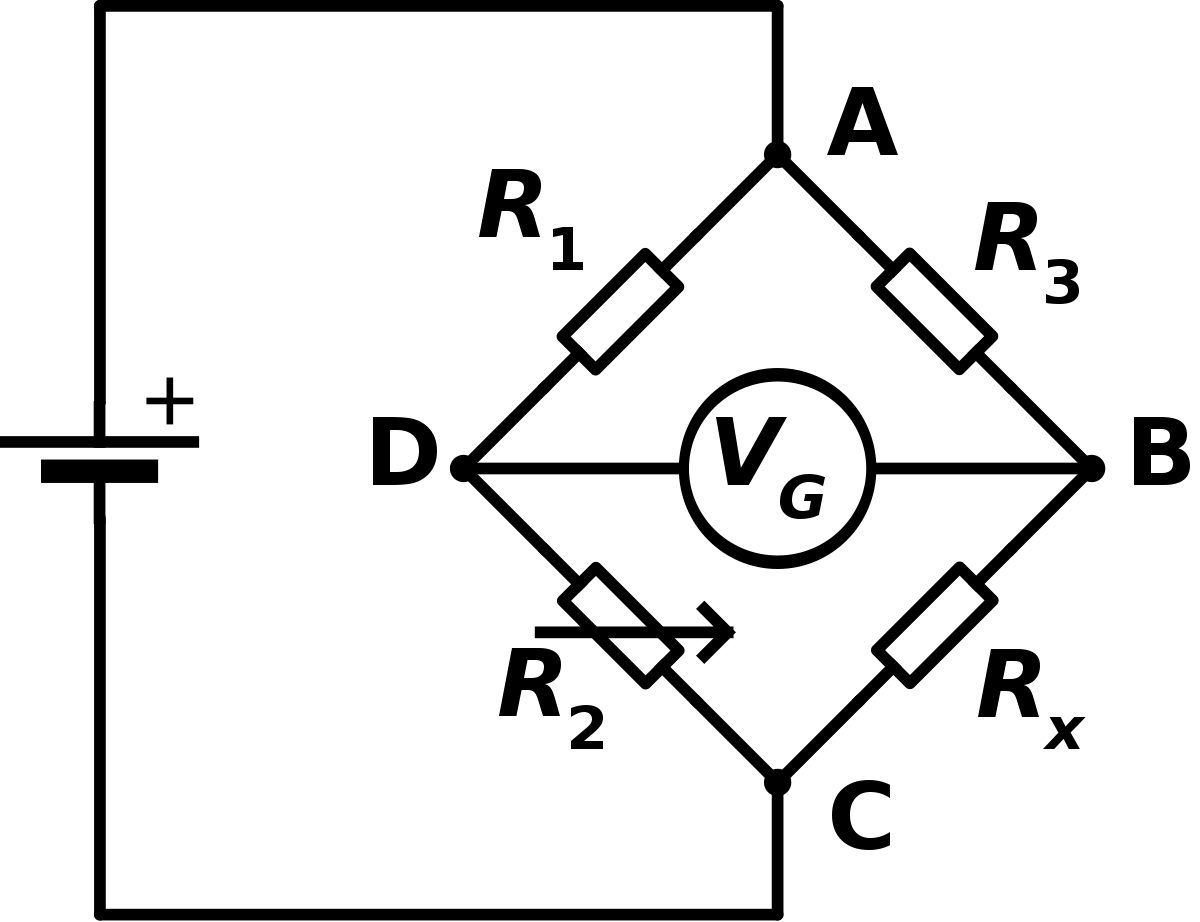
\includegraphics[scale=0.2]{1200px-Wheatstonebridge.png}
    \caption{Circuito "Puente de Wheatstone"}
    \label{fig:wheatstone}
\end{figure}

Durante los próximos años, el desarrollo de esta tecnología hace que se extienda moderadamente, sobretodo en la industria militar, la aviación y las empresas automovilisticas, pero estos dispositivos suponian una gran carga económica a las empresas debido a su elevado coste, por lo que no se extendieron tanto.

\subsubsection{Segunda era: 1936-1950}
En 1936\cite{50yearsof} se inventó el acelerómetro basado en un extensometro. Un extensometro es un sensor que mide la deformación usando el efecto piezoresistivo que posee el material del que está construido. Este efecto provoca que el material cambie de resistencia al ser sometido a una fuerza mecánica. Este tipo de dispositivos eran mucho más baratos y sencillos de hacer, por lo que hizo que se extendieran por todas las industrias que los necesitaban pero no podían justificar los precios anteriores. De hecho, varias empresas de aviación se hacían sus propios dispositivos de manera interna.

El mayor problema que presentaban este tipo de acelerometros es que ofrecían un rango de voltaje de 30mV, por lo que dependiendo de la aplicación, la proporcion ruido-medida era muy mala. Para mejorar esto, se hacían los extensómetros muy finos, para tener la mayor flexibilidad posible, lo que hacía surgir otro problema, la fragilidad del sistema. Para solucionar esto, se dio una vuelta de tuerca, añadiendo un fluido amortiguante en el sistema, que limitara los rangos de vibración a 0.707 del punto crítico. De esta forma, se mejoraba la respuesta en frecuencia en un factor 3 y se reducía la amplificación de la frecuencia resonante a la mitad. Este método tenía deficiencias, la mayor de ellas que debido a la introducción del amortiguador que provocó que la respuesta en frecuencia se hiciera muy dependiente de la temperatura, reduciendo la usabilidad de estos dispositivos a $\pm 20$ °C de la temperatura ambiente.

Todos estos problemas hicieron que se buscaran alternativas a esta tecnología. Además, tenían problemas para detectar las aceleraciones transitorias. Esto fue estudiado por Levi \textit{et al.}\cite{levy} en 1950 en un estudio encargado por la oficina nacional de estándares(ahora conocido como NIST, instituto nacional de estándares y tecnología) y financiado por la Marina estadounidense. 

\subsubsection{Tercera era: 1950-1991}

Estas limitaciones hicieron que se investigaran más a fondo otras tecnologías, entre ellas el efecto piezoeléctrico. El efecto piezoelectrico es similar, en parte, al piezoresistivo, al recibir una fuerza mecanica, el reacciona, pero  en este caso, tiende a separar las cargas entre las caras, creando una diferencia de potencial. Como vimos antes, los piezoresistivos cambiaban  su resistencia, y los piezoelectricos generan un voltaje. Una gran ventaja que tienen es que los voltajes generados tienen un valor absoluto alto, por lo que trabajar con ellos es mucho más sencillo y el ruido pasa a ser un problema menor. Además, las frecuencias resonantes son muy altas, por lo que no hace falta amortiguarlas.

Estos dispositivos piezoelectricos son los padres de nuestos sensores. Algunos materiales usados para construirlos eran ferroelectricos y cuarzo. Debido a la bajada de coste del sistema, empezó a surgir un mercado competitivo en el que varias empresaas estaban innovando constantemente.

\subsubsection{Cuarta era: 1991-?}

Con la llegada de la era digital y la miniaturización, los acelerómetros dieron su última evolución hasta ahora, los sensores MEMS. El primero, fue sacado al mercado en 1991, el ADXL 150. Los sensores MEMS tienen grandes ventajas frente al resto. Su tamaño es de escala micrometríca, por lo que son baratos de construir en masa y no ocupan mucho espacio. Son eficientes energéticamente hablando, ya que apenas consumen electricidad. Los acelerómetros MEMS utilizan materiales piezoeléctricos para realizar la misma medida que se haría con un sensor más grande de los anteriores, pero a escala microscopica. Para hacerse una idea, en la figura \ref{fig:acelerometro}, se muestra una imagen de un acelerometro MEMS, el ADXL 362, que mide 3x3.25x1.06 mm.

\begin{figure}[h]
    \centering
    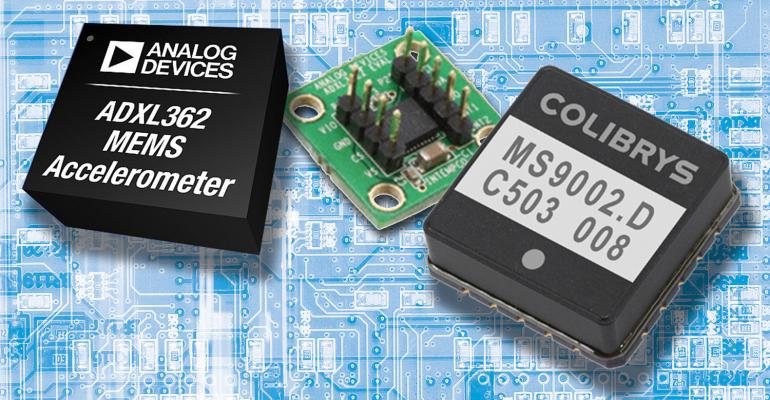
\includegraphics[width=1\textwidth]{MEMSpromo.jpg}
    \caption{Imagen de un acelerometro MEMS}
    \label{fig:acelerometro}
\end{figure}

\subsubsection{Conclusiones}

Desde inicio del siglo anterior ha sido un campo en constante avance, y sigue siendolo hoy en día. El desarrollo de los smartphones, videojuegos y nuevas tecnologías, que requerían acelerómetros cada vez más precisos no ha hecho sino ayudar a una tecnología que ya estaba presente en el campo militar, medico, de investigación, automovilistico... 

Hoy en día, los acelerómetros, y todo ese conjunto de sensores han cambiado nuestra forma de percibir el mundo. Con su ayuda, podemos realizar un control de pacientes, se pueden aplicar para mecanizar regadíos, para la conducción autónoma. Es una tecnología con muchos frentes de investigación y resulta muy interesante.

\subsection{Identificación de patrones movimiento}
Independientemente del tipo de movimiento que queramos estudiar, normalmente el proceso para la identificación de un patrón se divide en tres partes: Tomar medidas con los sensores, extraer la información relevante de esos datos y finalmente procesarla y clasificarla. Las dos últimas se hacen a nivel de software, por lo que a continuación se describe teniendo esto en cuenta con más detalle.

\subsubsection{Captura de información: Sensores}
Se van a enumerar los sensores de los que dispone un smartphone o un smartwatch cualquiera. Se hablará de sensores tipo MEMS. Estas siglas se refieren a \textit{microelectromechanical system}, o sistema microlectromecánico. Esto no es más que la miniaturización de los sistemas electrónicos.

\paragraph{Sensores de movimientos MEMS}

Al inicio, los smartphones tenían solo un sensor de movimiento MEMS, un acelerómetro. Este sensor mide la aceleración debida a la gravedad y al movimiento del cuerpo a través de tres ejes ortogonales. Con este sensor se han podido implementar algoritmos para ver el número de pasos. En los siguientes años se fue imponiendo sensor mas complejo, llamado IMU, \textit{inertial measurement unit}. Esta tiene 6 grados de libertad, 3 ejes de acelerómetro y otros 3 de giroscopio. El giroscopio se encarga de medir la velocidad angular de los tres ejes, y permite detectar el cambio de orientación del dispositivo. Y ya, en estos últimos años, esta IMU ha sido ampliada a MIMU, en la que se le ha añadido un magnetómetro, añadiendo 3 grados de libertad extra.

\paragraph{Sensores ambientales MEMS}

En el parrafó anterior se mencionó el magnetómetro, pero aunque está en el sensor de movimiento, es un sensor ambiental, ya que su medida depende de la posición del usuario con respecto al campo magnético terrestre. Así permite orientar el wearable con respecto al campo magnético de la tierra, y por tanto saber su posición exacta en reposo.

Además del magnetómetro, está el barómetro, que puede usar para determinar la diferencia de altura del usuario entre distintos momentos, o la presión ambiental, y saber la altura con respecto al mar a la que se encuentra.

Las ventajas de estos sensores es que no son invasivos y gasta poca batería su uso continuado, esto hace que sean ideales para hacer el sistema.
\paragraph{Sensores audiovisuales}

Aquí entran las cámaras y los micrófonos. Aunque útiles, en este trabajo no se hablará mucho de ellos, ya que aparte de gastar mucha batería, en el tema de la detección de patrones de movimiento no tienen mucho papel. Es cierto que se puede detectar distintos tipos de sonido, como hablar, musica, sonidos de ciudad etc \cite{Lu:2009:SSS:1555816.1555834}, y que se han usado las señales acústicas para detectar movimiento junto al giroscopio y acelerometro\cite{doi:10.1155/2014/503291}, pero al final los sensores MEMS son los que dominan.

\paragraph{Sensor de posición GPS}

Aparte de estos sensores, no hay que olvidarse del GPS. El GPS ha pasado de tener una precisión de 300m-1km\cite{vonWatzdorf:2010:APD:1899662.1899664} a tener precisión de metros en los últimos años\cite{s213}, donde con la ayuda de las redes móviles, la fuerza de la señal W-Fi y el bluetooth se alcanzan precisiones muy altas incluso en edificios y zonas de interior donde antes no era posible. Aunque tiene una carga de batería notable, también ofrece una información muy precisa y útil.

\paragraph{Sensor PPG}
Este sistema PPG(\textit{photoplethysmography}), fotopletismografía, aprovecha que la sangre absorbe el verde y rebota el rojo, y por tanto, usando luces led, se puede saber la cantidad de sangre que fluye por tu muñeca en un periodo de tiempo. Es fácil calcular el pulso pues en cada pulso va a haber un máximo de absorción/emisión. Este sistema se diferencia del habitual electrocardiograma(ECG) en que el electrocardiograma utiliza las señales eléctricas que reciben los músculos para hacer una contracción. El ECG es el método más preciso, pero en estudios recientes se ha visto que la diferencia entre uno y otro no es más de un 10\% \cite{77489867} en el peor de los casos, de forma que el método PPG tiene ciertas ventajas, principalmente la comodidad, ya que el usuario no necesita una banda con electrodos colocada alrededor del pecho.

Es un sistema localizado mas en smartbands o smartwatches que en smartphones, pero ofrece algo que los smartphones no pueden y es una información interesante.

\subsubsection{Desarrollo del algoritmo}
Inicialmente los modelos que se desarrollaban para ver el estado de movimiento eran clasificadores heurísticos, por ensayo y error. Esto se debía a que los smartphones iniciales tenían una capacidad de procesamiento limitada. Sin embargo, los smartphones modernos tienen la potencia como para ejecutar algoritmos modernos de extracción de datos y modelos de clasificación.

Estos modelos son entrenados con diversos MLAs(\textit{Machine learning algorithms}). Estos algoritmos analizan los datos de entrada durante un proceso supervisado de aprendizaje que defina la función o reglas que se usan para clasificar el movimiento, en este caso los distintos tipos que hay. Algunos de los MLAs usados son:

\begin{itemize}
\item Modelo oculto de Markov
\item K vecinos más próximos
\item Maquinas de vectores de soporte
\item Redes Bayesianas
\item Modelos gausianos de combinación
\item Regresiones logísticas
\item Clasificador bayesiano ingenuo
\item Árbol de decisiones
\item Redes neuronales.
\end{itemize}

\subparagraph{Modelo oculto de Markov} Este modelo asume que el sistema a estudiar es un proceso de Markov con parámetros desconocidos. Un proceso de Markov es un fenómeno aleatorio dependiente del tiempo para el cual se cumple la propiedad de Markov, que es que la variable a estudiar no tiene memoria. Esto implica que la probabilidad condicional sobre el estado presente, pasado y futuro son independientes.

\subparagraph{K vecinos más próximos} Es un modelo de reconocimiento de patrones. El caso de los más próximos es no parámetrico, ya que clasifica en función de la cercanía. Si es clasificador, la salida del modelo es la clase a la que pertenece. Si es de regresión, la salida es el valor de una propiedad del objeto estudiado. Ese valor es la media de los k vecinos más cercanos.

\subparagraph{Maquinas de vectores de soporte} Estos algoritmos son modelos de aprendizaje supervisado que analizan los datos y separan los datos en distintos sectores. A partir de ese entrenamiento, posteriormente se van separando los datos de entrada entre las distintas secciones.

\subparagraph{Redes Bayesianas} Son modelos probabilísticos de grafos, que representan unas variables, sus dependencias condicionales mediante un grafo directo. Un ejemplo seria las enfermedades y sus síntomas. Unos síntomas dados obtendrían la enfermedad que está afectando al individuo.

\subparagraph{Regresiones logísticas} Usa una función logística para obtener un modelo de varias variables.

\subparagraph{Clasificador bayesiano ingenuo} Es parecido al modelo de redes bayesianas, pero se simplifica haciendo que haya mas independencia entre las distintas clases de objetos a estudiar.

\subparagraph{Árbol de decisiones} Usa un árbol como modelo predictivo para obtener a partir de observaciones de un objeto conclusiones.

\subparagraph{Redes neuronales} Son un algoritmo basado en las neuronas. Aprenden independientemente a partir de un conjunto de datos de entrada a distinguir que es lo que los une o separa.

De entre todos estos, aquí se van a usar las redes neuronales, por eso se va a hacer una sección ampliando la información sobre éstas posteriormente. Se va a usar las redes neuronales porque se ha probado que son eficaces para este tipo de problemas\cite{s131013099} con eficacias de hasta el 87\%. Esto es así porque las redes neuronales son una herramienta muy potente para la clasificación o separación de distintos eventos. Son potentes aprendiendo patrones de comportamiento, y no los comportamientos en si, que es lo interesante aquí, ya que no todas las personas van a andar igual, o saltar o caerse de la misma forma, sin embargo los patrones si van a ser similares.

\subsubsection{Limitaciones}

Son muchos sensores de los que dispone un sistema android, usarlos todos en todo momento nos daría una imagen perfecta o casi perfecta de la situación de movimiento del usuario. Sin embargo usarlos todos constantemente tiene problemas. Nos centraremos aquí en el gasto de batería y en las limitaciones de los modelos.

\paragraph{Gasto de batería}
Hemos visto como se paso de baterías que duraban semanas en los antiguos Nokias a baterías de día y medio o menos, que es lo que ocurre habitualmente ahora. Poner a trabajar todos los sensores y el procesador con los datos es fatal para la duración de batería del dispositivo. Debido a ello se utilizan alternativas al recoger todo y analizar. 

Hablando de esto, se ha estudiado que hay tres factores que afectan al gasto de bateria de un smartphone, el primero es el numero de interacciones entre el usuario y el smartphone, el segundo las aplicaciones instaladas y usadas por el usuario y finalmente el hardware y el sistema operativo del terminal\cite{Falaki:2010:DSU:1814433.1814453}. Además, se ha estudiado que en estado de suspensión, pantalla apagada pero smartphone encendido el principal consumidor es el modulo GSM, el encargado de la conexión por datos a internet. Por el contrario, si el teléfono esta encendido, pero en idle, es decir, no tiene aplicaciones en segundo plano, es el procesador gráfico lo que más consume\cite{Carroll:2010:APC:1855840.1855861}. Se puede observar en la figura \ref{fig:consumo} gráficamente.
\begin{figure}[h]
    \centering
    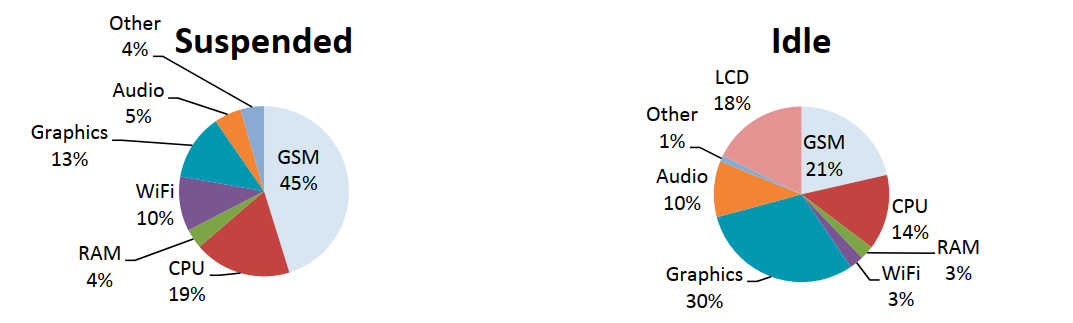
\includegraphics[width=1\textwidth]{batterylife.png}
    \caption{Gasto de bateria de un smartphone\cite{Carroll:2010:APC:1855840.1855861}}
    \label{fig:consumo}
\end{figure}

\paragraph{Modelos de posición fija}
Una limitación a la hora de modelar el movimiento de un usuario usando un smartphone es que su posición no es fija, puede estar en distintas partes del cuerpo, como se ve en la figura \ref{fig:posiciones}
\begin{figure}[h]
    \centering
    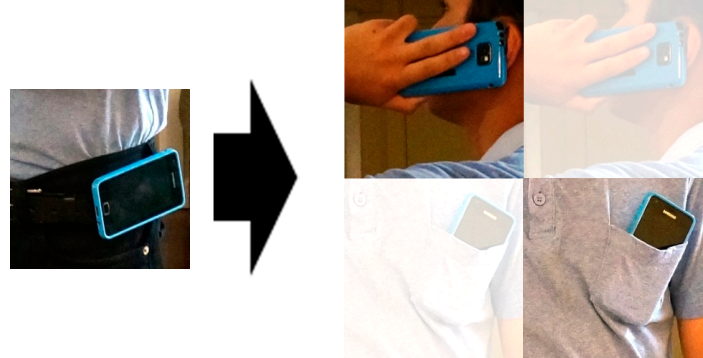
\includegraphics[width=1\textwidth]{position.png}
    \caption{Ejemplo de distintas posiciones de un smartphone.}
    \label{fig:posiciones}
\end{figure}

y nuestro algoritmo debe tenerlas en cuenta. Tienen ventajas e inconvenientes. 

Si se usa un algoritmo de posición fija, se obliga al usuario a tener que llevar el dispositivo de una determinada forma siempre, fijo, pero a cambio, al saber su posición exacta el algoritmo puede ser mucho mas preciso, ya que toma en cuenta principios de la biomecánica aplicados a esa zona concreta. Aunque si el objetivo es el estado de movimiento, el smartphone ha de estar lo más cerca posible del centro de masas, por eso la mayoria de los estudios tienen el smartphone fijo en un cinturón\cite{5673816}.

Se han hecho estudios aplicados a deportes y similares en los que al estar el dispositivo en una posición fija, se puede detectar perfectamente el tipo de movimiento. Hay aplicaciones aplicadas al futbol\cite{s130405317} y al hockey, a la natación\cite{Marshall:2013:SSD:2494091.2496036}, y como personal trainer en un gimnasio colocando el smartphone una tabla de equilibrios\cite{KRANZ2013203}.

\paragraph{Modelos de posición dependiente}

Estos modelos son una pequeña variación del anterior, en el cual se supone que el dispositivo va a estar alrededor de unas zonas concretas. Permiten que el dispositivo no esté absolutamente fijo, lo cual es una comodidad para el usuario. Además no pierden mucha exactitud. Estos modelos ya apenas se usan, fueron un avance del anterior en comodidad para el usuario, pero al final, son un parche sobre el problema, que lo alivia pero no lo soluciona. Los usuarios solo pueden tener el dispositivo en ciertas posiciones, no todas.

\paragraph{Modelos independientes de la posición}

En estos modelos, no importa la posición del dispositivo con respecto al usuario. Son los más cómodos para éste pero pierden capacidad. Por ejemplo, hay estudios en los que se detectan bien hasta siete tipos de movimiento, pero luego los estacionarios típicos como de pie, sentado y tumbado no es capaz de hacerlo\cite{6488584}.% 

\subsubsection{Conclusiones}

En nuestro caso, el algoritmo a utilizar es un modelo de posición fija, ya que es el evidente a usar en un smartwatch. El sensor que se va a utilizar es el acelerometro, porque es el que mejor se ajusta a las necesidades del proyecto, por los datos que ofrece y por el poco gasto de batería que produce. Y el sistema de aprendizaje se usará una red neuronal, ya que ha demostrado en estudios anteriores que es un algoritmo que ha sido probado ya en estudios anteriores.


\newpage
\section{Fundamentos teóricos}
\subsection{Introducción a las redes neuronales}
\subsubsection{Definición}
Las redes neuronales son una herramienta matemática basada vagamente en una neurona. Son redes de elementos que utilizan algoritmos de aprendizajes.

\subsubsection{Estructura biológica}

\begin{figure}[h]
    \centering
    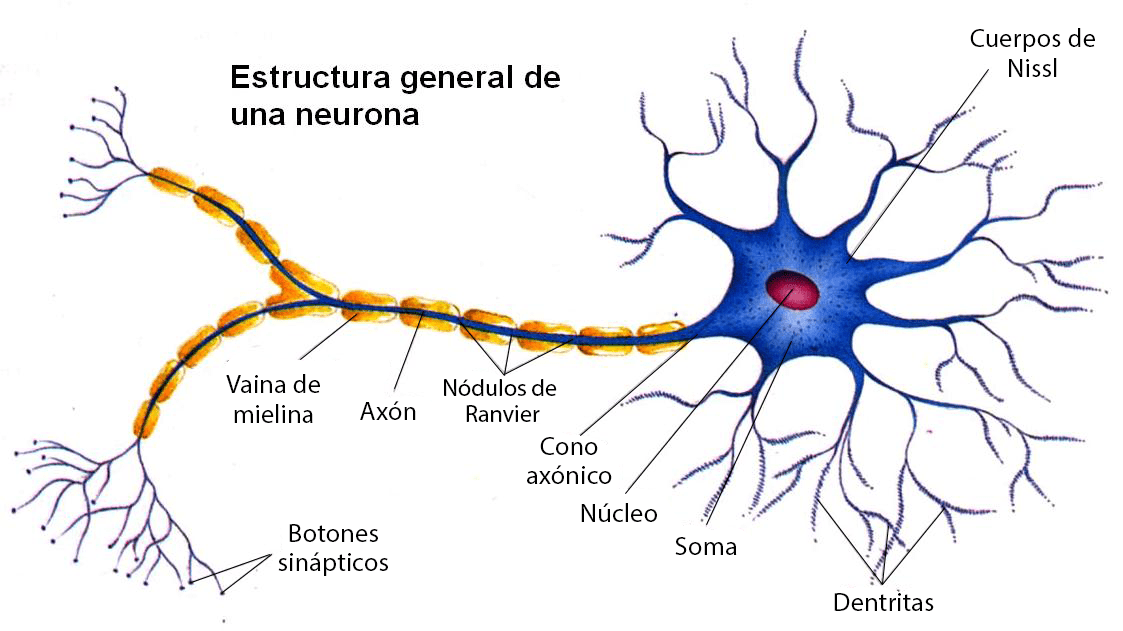
\includegraphics[width=1\textwidth]{estructura_general_neurona.png}
    \caption{Estructura del una neurona.}
    \label{fig:neuronareal}
\end{figure}

Se puede observar en la figura \ref{fig:neuronareal} que una neurona es muy distinta a la célula típica. Lo más importante de una neurona es que está unida a otras muchas mediante las dendritas y los botones sinápticos. La neurona se excita por las dendritas mediante un proceso llamado sinapsis, que consiste en el intercambio de neurotransmisores en ellas. Esto provoca un impulso nervioso, que se transmite posteriormente por el axón hasta los botones sinápticos, que están conectados a otras neuronas o músculos.

El axón es el elemento alargado, rodeado por vainas de mielina y éstas acaban en los nódulos de Ranvier. Las vainas de mielina son células de Schwann y actúan de encapsuladores de la señal, haciendo que la señal no se pierda. Los nódulos de Ranvier son los huecos que quedan en el axón entre células de Schwann. Estos 'huecos' están llenos de iones que amplifican la señal.

\begin{figure}[h]
    \centering
    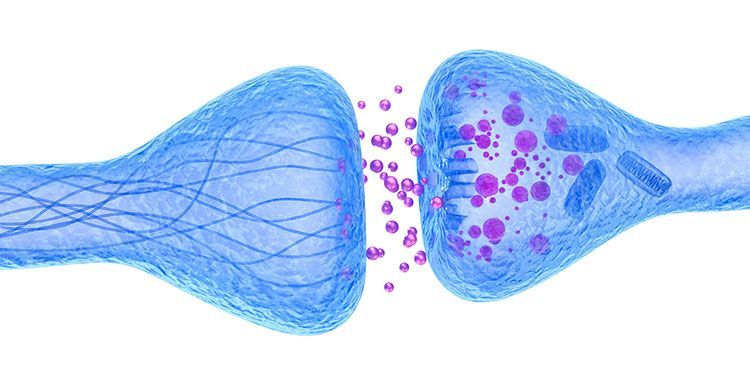
\includegraphics[width=0.8\textwidth]{sinapsis.jpg}
    \caption{Sinapsis de una neurona.}
    \label{fig:mesh2}
\end{figure}

Además, las neuronas tienen un comportamiento más a tener en cuenta. No están constantemente trabajando, sino que tienen fases de descansos. A estas fases se le llaman estado refractario. Es el tiempo necesario tras una estimulación necesario para recuperar el estado inicial previo y en el cual no puede volver a ser excitada. Se puede ver en la figura \ref{fig:refractario} las fases de activación de una neurona
\begin{figure}[h]
    \centering
    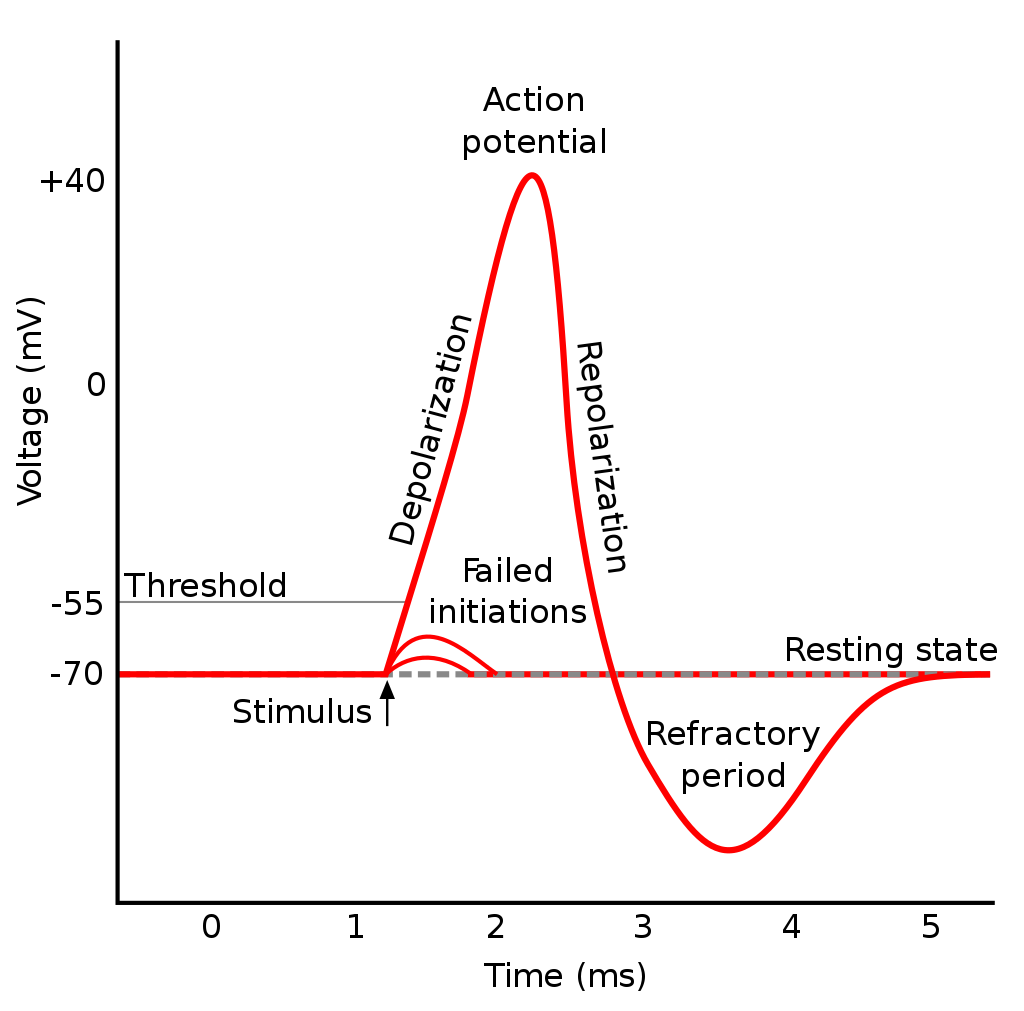
\includegraphics[scale=0.2]{refractorystate.png}
    \caption{Estado refractario.}
    \label{fig:refractario}
\end{figure}

Que en una neurona suele durar 1 mili segundo. Todo esto hace que las neuronas sean una célula de especial interés, ya que tiene una estructura interesante que puede ser reproducida matemáticamente y algorítmicamente, aunque evidentemente las neuronas reales son más complejas que las de los algoritmos.

La sinapsis es el proceso más importante, ya que el 'peso' de cada sinapsis, y a quien se tiene que transmitir esa señal es decidido en la neurona muy rápidamente. Además, la sinapsis tiene distintos orígenes, químicos o eléctricos. La neurona puede trabajar con neurotransmisores que son sustancias químicas como la dopamina, o puede ser eléctrica directamente, mediante la transmisión directa de iones.	

Además, la sinapsis puede tener tres clases, excitadora, que incrementa la energía, 	inhibidora, que la reduce y moduladora, que es la que cambia el patrón o la frecuencia de la actividad de la que se ocupe ese grupo de neuronas. 

\subsubsection{Estructura en el software}

El interés en las redes neuronales lleva tanto como la computación moderna. Los algoritmos son antiguos pero siempre ha existido la limitación en el hardware, ya que los algoritmos consisten en muchos elementos trabajando en paralelo. Los primeros algoritmos son de los 50-60. El más importante de ellos es el de Perceptrón. El Perceptrón es un algoritmo de aprendizaje supervisado de un clasificador binario. Esto es, un algoritmo que dependiendo de la entrada, puede decidir la clase de elemento que es. Fue inventado por Rosenblatt como una estructura monocapa con una función de activación estilo escalón.

La función de activación es la que define el comportamiento de una neurona. De la función de activación depende el funcionamiento de la neurona y sobretodo los resultados que da. En una función escalón el resultado va a ser Si o No, 0 ó 1. Sin embargo, la función puede ser Gaussiana, la identidad, una tangente... Depende del problema a resolver y del algoritmo.

A partir del algoritmo del perceptrón se desarrolla en los 80 el perceptrón multicapa. Este es el algoritmo más importante del campo, y tiene ya 40 años. Este algoritmo tiene una capa de entrada, una de salida y las que sean necesarias entre media.

\begin{figure}[h]
    \centering
    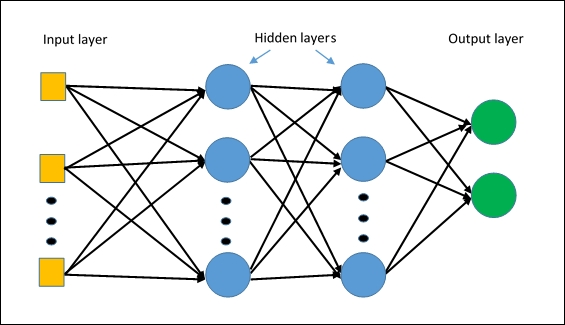
\includegraphics[width=0.7\textwidth]{multicapa.jpg}
    \caption{Estructura de un perceptrón multicapa.}
    \label{fig:estructuraneurona}
\end{figure}

La estructura del algoritmo es similar a la de la figura \ref{fig:estructuraneurona}, donde lo más importante es que cada neurona está conectada a todas las neuronas de la capa anterior y posterior. Lo interesante de este algoritmo es que cada capa puede tener una función de activación distinta y ocuparse de una función distinta. Al ser muy genérico, el perceptrón multicapa puede ser usado en muchos problemas simplemente adaptando el número de capas internas o la función que cumplen. Hasta hace poco, hacer un modelo con mucha profundidad de capas era muy caro a nivel de hardware, pero con el aumento de potencia y de la potencia en la nube, ha hecho que resurja el campo de investigación, mas centrado en la resolución de problemas complejos y muchas capas para ello, conocido como \textit{deep learning}. La limitación de hardware ha sido ahora sustituida por una computación en la nube muy barata que se puede alquilar a Amazon Cloud o Google y ha revolucionado el campo.

\begin{figure}[h]
    \centering
    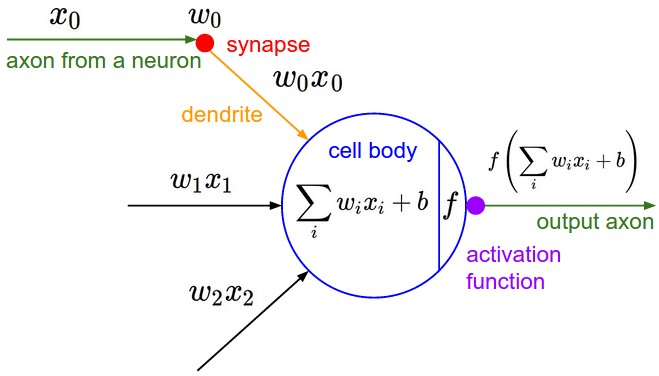
\includegraphics[width=0.7\textwidth]{neuron.jpg}
    \caption{Estructura de una neurona.}
    \label{fig:estructura}
\end{figure}

El funcionamiento básico de cada elemento en una red es similar al de la figura \ref{fig:estructura}, cada 'neurona' le llegan los axones de otras neuronas(la capa anterior a ella) con unos valores $x_0$ sobre los que se aplica un peso $w_0$, de forma que se normaliza, y luego se ve si activa la función de activación y se transmite a las neuronas de las siguientes capas por su 'axón'. El valor b es un umbral, que sirve para cambiar el punto de activación.

La capacidad de aprender de la neurona consiste en preparar los pesos $w_i$ en un proceso de entrenamiento. En los pesos sinápticos es donde está la profundidad del tema. Hay dos formas de entrenar una neurona, mediante un aprendizaje supervisado o mediante un aprendizaje no supervisado. El caso del aprendizaje supervisado, se entrega a una red neuronal los datos de entrada y de salida y mediante el proceso de aprendizaje adapta los pesos para obtener los resultados. En el caso de un aprendizaje no supervisado, se le dan los datos y la red lo clasifica ella sola. Lo importante en el caso del aprendizaje supervisado es entregar unos buenos datos clasificados, y en el caso de un aprendizaje no supervisado, lo importante es el análisis posterior, ver en que se ha basado la red para clasificarlos, que a veces es de formas que no se esperan.

\subsubsection{Algoritmo de entrenamiento: Backpropagation}
Para entrenar la red se utiliza un algoritmo conocido como \textit{backpropagation}, o en español retropropagación. Esto es así porque se entrena primero a la capa más profunda(la más cercana a la salida) y posteriormente se van ajustando los errores de la anterior.

El aprendizaje consiste en introducir los datos de entrada, comparar con los de salida y ver el error cometido. Posteriormente se intenta minimizar ese error. El aprendizaje pues es ajustar los pesos sinápticos para minimizar el error. El aprendizaje puede hacerse de dos formas, por lotes se hace un error global al presentar todos los patrones, y incremental, en el que se presentan los patrones uno a uno	y se adaptan los pesos a cada patrón. Nuestros datos son:

\begin{equation}
x^P = [x_i^P] \; i= 1,..., N_e
\end{equation}
\begin{equation}
d^P = [d_k^P] \; k=1,...,N_s
\end{equation}

Donde las X son un conjunto de datos de entrada, y las D la salida para el conjunto de datos de entrada anterior. $N_s$ representa el número de salidas y $N_e$ el número de entradas. Ademas, al valor b, umbral, se le considera un peso más, $w_0$. Para empezar, se le entrega a la red el patrón de entrada $x^P$, y se obtiene una salida:

\begin{equation}
y_k^P=\Psi _s(z^P_k)=\Psi _s
\end{equation}

Donde $\Psi$ es la función de activación de la ultima capa. Ahora se compara cada dato con el valor de salida real, y se obtiene un error:

\begin{equation}
e^P_k=d_k^P-y_k^P
\end{equation}

El error global obtenido tiene en cuenta el de todas las neuronas, y se representa de forma cuadrática:

\begin{equation}
E^P = \frac{1}{2} \sum_{k=1}^{N_s} (e_k^P)^2=\frac{1}{2}\sum_{k=1}^{N_s}(d_k^P-y_k^P)^2
\end{equation}

Y finalmente se modifican los pesos sinápticos para minimizar el error:

\begin{equation}
w_{kj}(t+1)=w_{kj}(t) + \Delta w_{kj}(t+1)
\end{equation}

La forma de calcular $\Delta w_{kj}(t+1)$ es la que define al algoritmo de adaptación(aprendizaje). El algoritmo debe modificar todos los pesos de todas las neuronas de todas las capas de la red. Como solo se conoce el error en la salida, es necesario empezar por el final, a continuación se calculan los errores de la capa anterior, donde se considera el resultado obtenido en la capa de salida como el correcto y se ve el error con el calculado en la capa anterior. Así, sucesivamente, se llega hasta la primera capa. Esta forma de calcular es la que hace que se llame al método \textit{Backpropagation}. 

Primero hay que ver como varía el error en función de los pesos. Para ello hacemos el gradiente de la función de error respecto a los pesos

\begin{equation}
\nabla E^P = \frac{\partial E^P}{\partial w_{kj}}
\end{equation}

Aplicamos la regla de la cadena:

\begin{equation}
\frac{\partial E^P}{\partial w_{kj}} =  \frac{\partial E^P}{\partial e_{k}^P} \frac{\partial e^P_k}{\partial y_{k}^P} \frac{\partial y^P_k}{\partial z_{k}^P} \frac{\partial z^P_k}{\partial w_{kj}}
\end{equation}

El valor del primer termino es:

\begin{equation}
\frac{\partial E^P}{\partial e_{k}^P} =  \frac{\partial}{\partial e_k^P}\left(\frac{1}{2} \sum_{k=1}^{N_s} (e_k^P)^2\right) = e^P_k=(d_k^P-y_k^P)
\end{equation}

El segundo:

\begin{equation}
\frac{\partial e^P_k}{\partial y_{k}^P} = \frac{\partial}{\partial y_{k}^P}\left(d^P_k - y^P_k\right) = -1
\end{equation}

Tercero: 

\begin{equation}
\frac{\partial y^P_k}{\partial z_{k}^P} = \frac{\partial \Psi _s(z_k^P)}{\partial z_{k}^P} = \Psi _s'(z_k^P)
\end{equation}

Finalmente, el cuarto:

\begin{equation}
\frac{\partial z^P_k}{\partial w_{kj}}=\frac{\partial \left(\sum_{j=0}^{N_e} w_{kj} y_j^P\right)}{\partial w_{kj}} = y_j^P
\end{equation}

Recomponiendo se llega a:

\begin{equation}
\frac{\partial E^P}{\partial w_{kj}} =
-(d_k^P-y_k^P) \cdot \Psi _s'(z_k^P) \cdot y_j^P
\end{equation}

Ahora se define la sensibilidad de la neurona k-esima ante el patrón de entrada P($\delta_k^P$) como:

\begin{equation}
\delta _k^P = - \frac{\partial E^P}{\partial e^P_k}=-
\frac{\partial E^P}{\partial e_{k}^P} \frac{\partial e^P_k}{\partial y_{k}^P} \frac{\partial y^P_k}{\partial z_{k}^P} = (d_k^P-y_k^P) \cdot \Psi _s'(z_k^P)
\end{equation}

De forma que finalmente, la expresión del gradiente de error queda como:

\begin{equation}
\frac{\partial E^P}{\partial w_{kj}} = \delta_k^P \cdot y_j^P
\end{equation}

Para que la variación del peso haga disminuir la función de error, el error ha de ser proporcional al gradiente negativo de la función de error respecto a los pesos:

\begin{equation}
\Delta w_{kj}(t+1) = -\eta \frac{\partial E^P}{\partial w_{kj}} = \eta \delta_k^P y_j^P
\end{equation}

Donde $\eta$ es una constante de proporcionalidad cuyo valor se ajusta para adaptar la velocidad y precisión del aprendizaje. Con esto tenemos el algoritmo de la capa de salida. Ahora para hacer la ultima capa oculta, que no tiene ninguna dificultad desde el punto conceptual, pero si matemática:

\begin{multline}
E^P = \frac{1}{2} \sum_{k=1}^{N_s} (e_k^P)^2=\frac{1}{2}\sum_{k=1}^{N_s}(d_k^P-y_k^P)^2 =  \frac{1}{2} \sum_{k=1}^{N_s} \left(d_k^P - \Psi _s(z_k^P)\right)^2 =\\
\quad = \frac{1}{2} \sum_{k=1}^{N_s} \left(d_k^P - \Psi _s \left[ \sum_{j=0}^{N_s} w_{kj} y_j^P\right]\right)^2 = \\
\qquad \qquad = \frac{1}{2} \sum_{k=1}^{N_s} \left(d_k^P - \Psi _s \left[ \sum_{j=0}^{N_s} w_{kj}\Psi _{s-1}(z_j^P)\right]\right)^2 =\\
= \frac{1}{2} \sum_{k=1}^{N_s} \left(d_k^P - \Psi _s \left[ \sum_{j=0}^{N_s} w_{kj}\Psi _{s-1} \left\langle \sum_{l=0}^{N_s'} w_{jl} y_l^P\right\rangle \right] \right)^2
\end{multline}

A partir de esta expresión, se puede obtener, para el cálculo del gradiente del error:

\begin{equation}
\frac{\partial E^P}{\partial w_{jl}} = \frac{\partial E^P}{\partial e_{k}^P} \frac{\partial e^P_k}{\partial y_{k}^P} \frac{\partial y^P_k}{\partial z_{k}^P} \frac{\partial z^P_k}{\partial y_j^P} \frac{\partial y^P_j}{\partial z_j^P} \frac{\partial z^P_j}{\partial w_{jl}}
\end{equation}

Y calculando las derivadas, como en el caso anterior, una a una, se llega a:

\begin{equation}
\frac{\partial E^P}{\partial w_{jl}} =-\sum _{k=1}^{N_s}(d_k^P-y_k^P) \cdot \Psi ' _s(z_k^P) \cdot w_{kj} \cdot \Psi '_{s-1}(z_j^P) \cdot y_l^P
\end{equation}

Definiendo de nuevo la sensibilidad:

\begin{equation}
\delta _j^P = -\sum _{k=1}^{N_s}(d_k^P-y_k^P) \cdot \Psi ' _s(z_k^P) \cdot w_{kj} \cdot \Psi '_{s-1}(z_j^P)
\end{equation}

Obtenemos, finalmente:

\begin{equation}
\frac{\partial E^P}{\partial w_{jl}} = \delta _j^P \cdot y_l^P
\end{equation}

Y el resultado de la variación de pesos sería: 

\begin{equation}
\Delta w_{jl} = -\eta \frac{\partial E^P}{\partial w_{jl}} = \eta \cdot \delta _j^P \cdot y_l^P
\end{equation}

De esta forma se va iterando de forma que cada neurona de cada capa tiene una sensibilidad distinta adaptada a ella.

\subsection{Acelerometros}

Empecemos por la máquina de Atwood, que es un ejemplo clásico de acelerómetro. Como se mostró en la figura \ref{fig:atwood}, el sistema es sencillo, dos masas conectadas por una cuerda. De esta forma, las ecuaciones que afectan a cada masa son:

\begin{equation}
m_1 g -T = m_1 a
\end{equation}
\begin{equation}
T - m_2 g = m_2 a
\end{equation}

De esta forma, si se suman ambas ecuaciones:

\begin{equation}
(m_1 -m_2)g = (m_1+m_2)a
\end{equation}

Y conociendo las másas y la aceleración de la gravedad, se puede obtener la aceleración simplemente despejando.

Un acelerómetro digital no es muy distinto, se puede ver un diagrama en la figura \ref{fig:piezoelectric}

\begin{figure}[h]
    \centering
    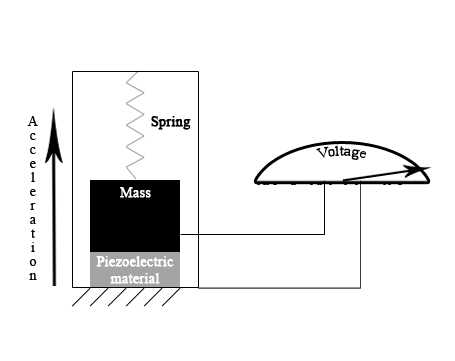
\includegraphics[scale=0.8]{piezoelectric.png}
    \caption{Acelerómetro piezoelectrico.}
    \label{fig:piezoelectric}
\end{figure}

Un acelerómetro piezoeléctrico se basa en las propiedades de este material. La propiedad que da nombre al material es que en él su estructura interna cambia cuando es sometido a una fuerza. Las cargas que posee se acumulan en sus caras, separadas entre si, creando una diferencia de potencial y por tanto un voltaje. De esta forma, sabiendo el voltaje produido y las constantes del sistema se puede obtener el parámetro deseado, como se puede observar en la figura \ref{fig:piezotypes}.

\begin{figure}[h]
    \centering
    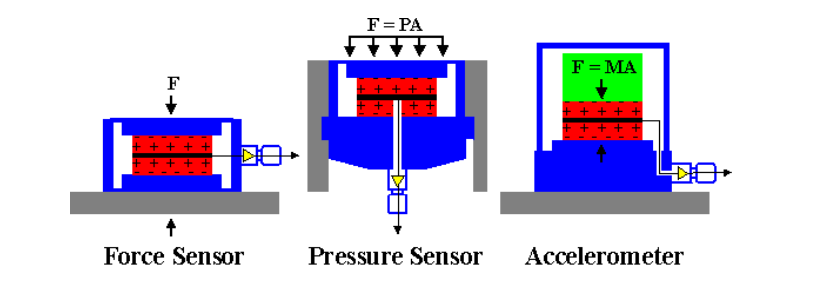
\includegraphics[width=1\textwidth]{piezoelectrictypes.png}
    \caption{Distintos tipos de dispositivos piezoelectricos.}
    \label{fig:piezotypes}
\end{figure}

Como se ve, los dispositivos piezoelectricos tienen muchas aplicaciones. Además producen bastante voltaje con poca fuerza aplicada a ellos, y ofrecen un comportamiento lineal en un gran rango de fuerzas ejercidas sobre ellos. De esta forma, un sistema bien diseñado podría medir desde 0.0001 la fuerza de la gravedad hasta 100 o más veces la fuerza de la gravedad.
\newpage
\section{Descripción del sistema}
Ahora vamos a hablar del sistema en el que se realiza el estudio. El sistema cuenta con dos dispositivos físicos, un smartphone y un smartwatch. Estos dispositivos usan ambos android. En su versión para wearables, android se llama wearOS en el smartwatch
\subsection{Smartphone}
El smartphone elegido es Xiaomi Redmi note 5 pro. La elección es irrelevante ya que el smartphone se encarga únicamente en recibir datos y guardarlos. Es por esto que la elección del dispositivo no tiene mucha importancia ya que no requiere mucha potencia.
\subsection{Smartwatch}
El smartwatch por el contrario si tiene cierta importancia. El modelo exacto es Ticwatch E. Es un modelo de gama baja/media, con un precio contenido para las prestaciones que ofrece, pero interesante por ello. Al no ser un dispositivo caro, es accesible a un publico mayor. Además, es sencillo y discreto. Todo esto hace que sea una buena elección. En la figura \ref{fig:ticwatch} se puede observar el dispositivo.

\begin{figure}[h]
    \centering
    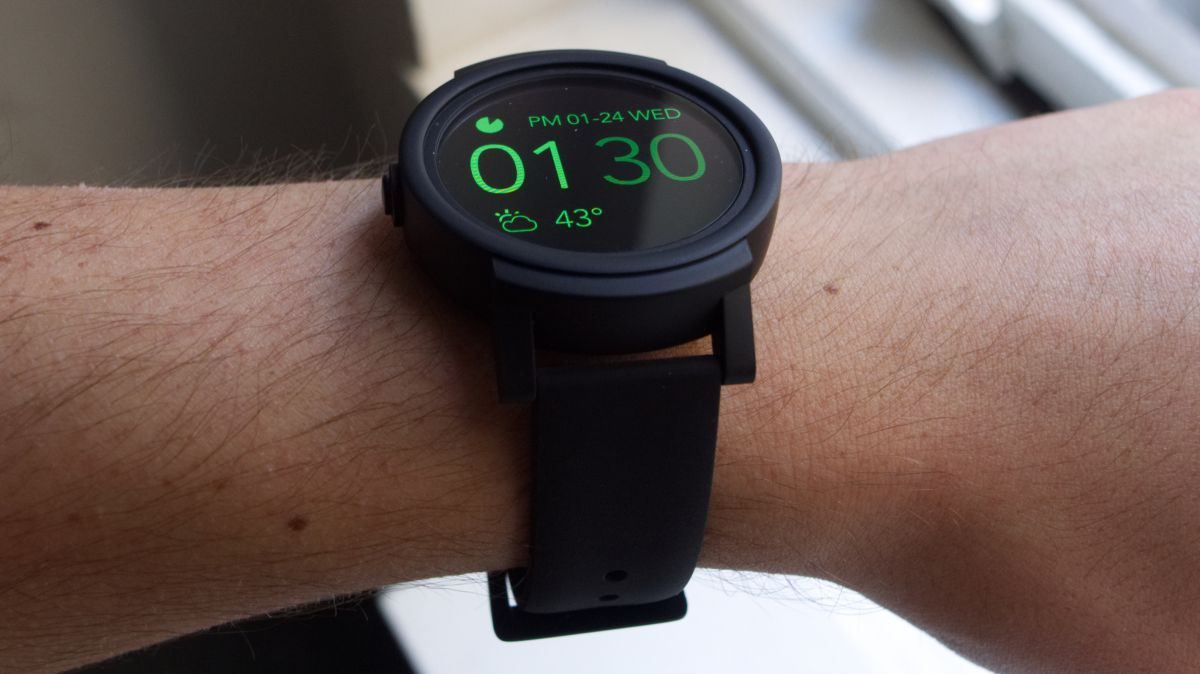
\includegraphics[width=1\textwidth]{ticwatche.jpg}
    \caption{Ticwatch E versión negra.}
    \label{fig:ticwatch}
\end{figure}

En las características técnicas, es un dispositivo con un procesador de doble núcleo a 1.2 GHz, MTK MT2601, basado en ARM Cortex-A7. Esto implica que es un procesador de bajo consumo y potencia moderada. La memoria RAM es de 512mb y la memoria ROM son 4Gb. Suficiente para un dispositivo de estas características. Para el GPS admite varios sistemas, GPS, GLONASS y Beidou. GLONASS es el GPS de Rusia y Beidou el de China. Tiene Bluetooth 4.1 BLE, que está especializado para aplicaciones al Internet of Things(IoT) por su bajo consumo. Respecto al resto de sensores, posee acelerómetro, giroscopio, sensor de proximidad, brújula electrónica y monitor del pulso.

\subsection{Software}

\subsubsection{Android Studio}

Android Studio es el IDE que recomienda Google para programar dispositivos basados en Android. Está desarrollado por IntelliJ, y es similar a sus otros productos como pueden ser Idea(Java), Pycharm(Python), PHPstorm(PHP). La interfaz es intuitiva y muy completa.

En este caso, para programar ambas cosas, hay que crear un proyecto adecuado para ello. En la pantalla inicial hay que seleccionar una versión objetivo, y el dispositivo para el que está desarrollado. En este caso la versión mínima es Android 6.0 \textit{Marshmallow}, que ofrece un 62.6\% del mercado como objetivo, y solo puede aumentar. Se ha elegido esta versión como base porque ofrece aún un buen arco de tiempo en el que Google Play Services ofrece cobertura, porque es una versión que modernizó el estilo de crear aplicaciones en Android, con la petición de permisos individuales, que hay que programar de todas formas para versiones 6.0 o superior. Además, la mayoría del entorno Android de aquella época sigue funcional. Esto es importante ya que Android es un sistema operativo en constante cambio, lo que implica que muchas funciones son sustituidas por otras más modernas, y acaban desfasadas. Todo esto hace que la versión mínima sea \textit{Marshmallow}.

Eso en el smartphone. En el smartwatch, la versión mínima ha de coincidir con la del teléfono, pero es menos importante, ya que aunque Google actualice todos sus dispositivos a la vez, y haga un Android 7.0 para smartphones y para smartwatches, los cambios son más livianos en el sistema operativo de los smartwatches.


\subsubsection{Matlab}

Matlab(Matrix Laboratory) es un idioma de programación orientado a cálculos matemáticos y especializado en cálculo con matrices, de forma nativa. En Matlab no existen arrays, existen Matrices de 1 columna o una fila, no existen variables, existen matrices 1x1. Esto hace que en el tratamiento de grandes volúmenes de datos sea una herramienta muy potente donde otros idiomas cojean. Matlab fue creado en los 70 para evitar tener que usar Fortran, en la universidad de Nuevo México. Rápidamente se extendió en el ambiente académico y a partir de 1984 se unieron sus creadores para comercializarlo. 

En Matlab todo es sencillo, introducir una matriz es tan sencillo como:
\lstset{language=matlab}
\begin{lstlisting}
A = [16 3 2 13; 5 10 11 8; 9 6 7 12; 4 15 14 1]
\end{lstlisting}

Esto es un paso gigantesco en comparación a otros idiomas de programación. Además, la gran ventaja de Matlab son su infinidad de paquetes especializados en ciencia. En este trabajo se usa la \textit{Deep Learning Toolbox}, la caja de herramienta de inteligencia artificial, con una interfaz gráfica que la hace muy sencilla de utilizar.

\subsection{Red Neuronal}

Para la red neuronal se ha utilizado la herramienta de Matlab de \textit{Deep Learning Toolbox}\cite{Matlab}. El tipo de red elegida es  \textit{Pattern recognition}, reconocimiento de patrones. En nuestro caso es el mejor método disponible, un aprendizaje supervisado que busca patrones para clasificar. De las cuatro opciones que ofrece la herramienta es la más adecuada aunque la otra opción interesante sería una \textit{Clustering App}, cuya principal diferencia con nuestra red es que es un aprendizaje no supervisado, por tanto, más expuesto a errores. Ya que los datos están clasificados al tomarlos, no tiene mucho sentido perder precisión sin ganar nada a cambio. En un caso con más tipos de movimientos si sería un tipo de red interesante.

Los otros casos se centran en buscar series temporales, la ecuación que pueda ajustarse, pero en este caso no es algo interesante.

La red entrenada es similar a la de la figura \ref{fig:redneuronal}

\begin{figure}[h]
    \centering
    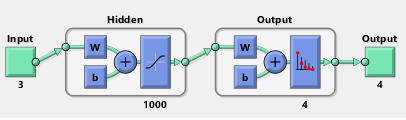
\includegraphics[width=1\textwidth]{redneuronal.png}
    \caption{Red Neuronal.}
    \label{fig:redneuronal}
\end{figure}

La red entrenada es similar a la de la figura \ref{fig:redneuronal}. Como se puede observar tiene 3 inputs, los 3 valores del acelerómetro y cuatro de salida, los cuatro tipos de movimientos, y con una sola capa oculta con 1000 neuronas y una función de activación tipo tangente hiperbólica.

El número de neuronas de la capa oculta es 1000. Para llegar a este número se ha ido iterando con distintos números, hasta llegar a un resultado aceptable. Con más neuronas la red se vuelve inútil ya que empieza a detectar datos mal, y con menos no alcanza tanta precisión.


\newpage
\section{Metodología}
Primero, se toman los datos de varios usuarios con el smartwatch, se recogen los datos con el smartphone y se procede a su análisis. Lo primero que se ve es que ni sus gráficas, ni el análisis de Fourier recoge información interesante.

\subsection{Toma de datos}

Para la toma de datos se ha usado una aplicación creada especialmente para esto en Android y Android Wear. La interfaz es mínima pues se ha considerado una aplicación experimental.

\begin{figure}[h]
    \centering
    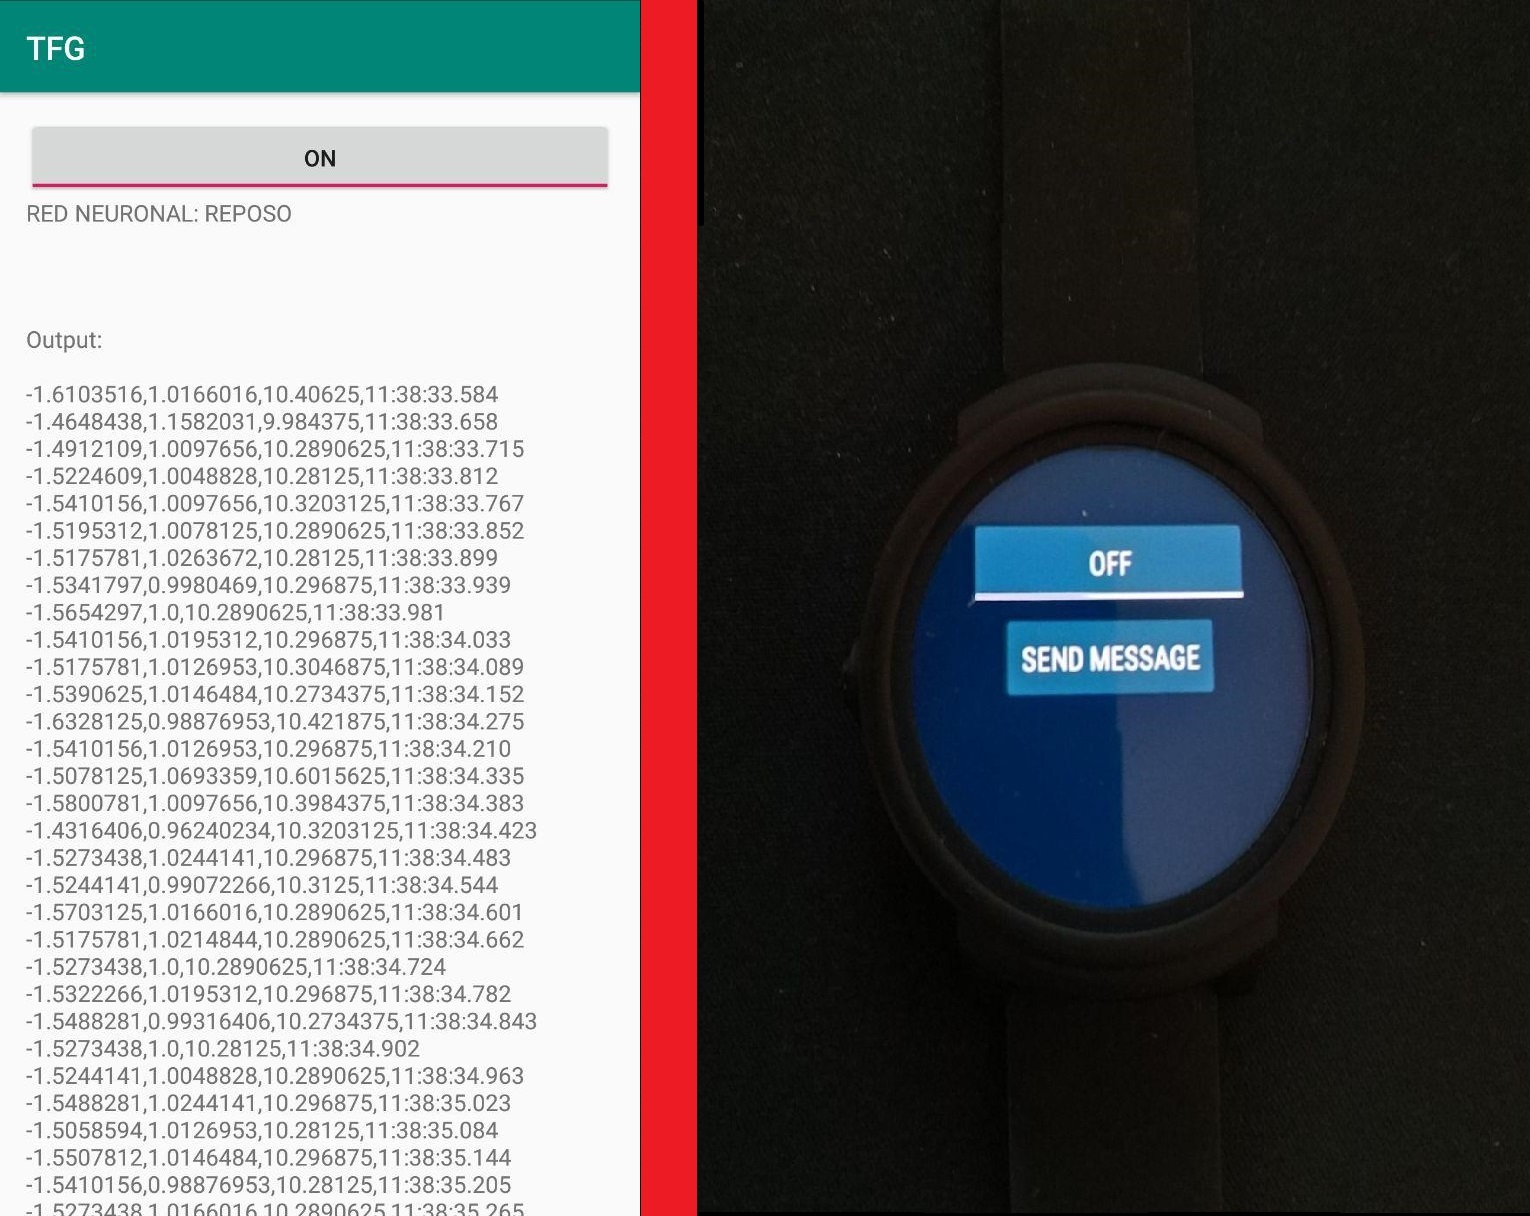
\includegraphics[width=0.8\textwidth]{Interfaces.jpg}
    \caption{Interfaz del smartphone y smartwatch.}
    \label{fig:mesh2}
\end{figure}

El botón del smartwatch de "Send Message" se ocupa de testear la conexión. En ambos hay un On y un Off que sirve para, en el caso del smartwatch para activar la transmisión de los datos del acelerómetro al móvil, y en el smartphone, al activarlo se empiezan a guardar, recibirse se reciben siempre y se actualizan en la lista de debajo. De esta forma, al tomar los datos el usuario tiene el control total de lo que ocurre con ellos.

Una vez solventado esto, para la toma de datos se hizo de la siguiente forma:

\begin{center}
\begin{table}
\caption{Metodología toma de datos}
\begin{tabular}{| c | c |}
\hline
Reposo & Toma de datos sentado y quieto. \\
\hline
Andando & Una vuelta a la manzana. \\
\hline
Corriendo & Dos vueltas a la manzana. \\
\hline
Cayendo & Colchón y dejarse caer, parando entre cada caída la toma de datos. \\
\hline
\end{tabular}
\label{tabla1}
\end{table}
\end{center}

En el cuadro \ref{tabla1} se puede ver que se ha dado vueltas a una manzana, en concreto, en la figura \ref{fig:cuadra} se puede observar:

\begin{figure}[h]
    \centering
    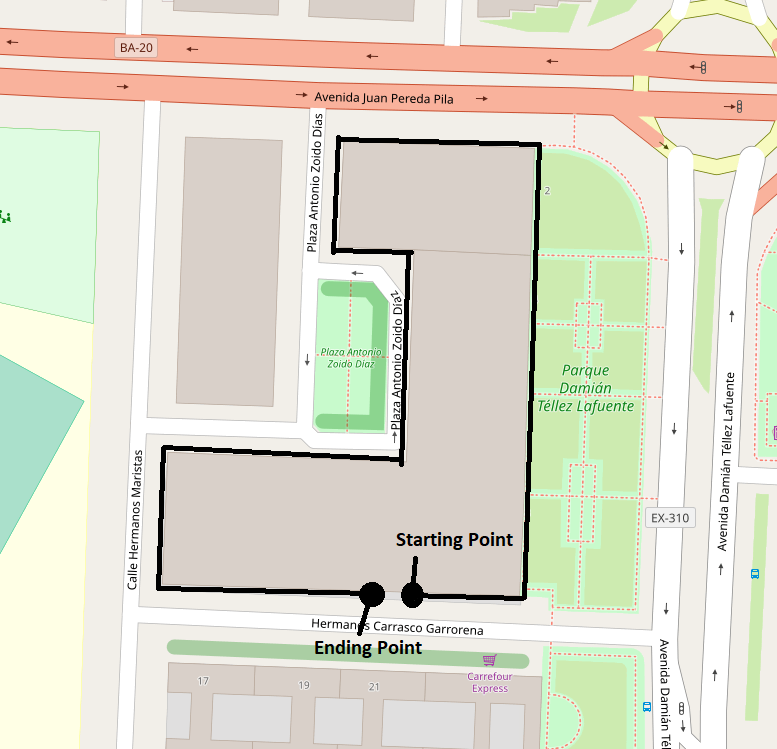
\includegraphics[width=0.6\textwidth]{plaza.png}
    \caption{Ruta toma de datos.}
    \label{fig:cuadra}
\end{figure}



\subsection{Análisis de los datos}
Primero se procederá a una enumeración de los datos obtenidos seguidos de un pequeño análisis.

A continuación se van a exponer las gráficas obtenidas para cada caso, y su transformada de Fourier.

\newpage

\subsubsection{Reposo}

Se representa en el primer caso cada variable en el eje Y y en el eje X es el numero de muestra correspondiente, lo que seria el tiempo.

\begin{figure}[h]
    \centering
    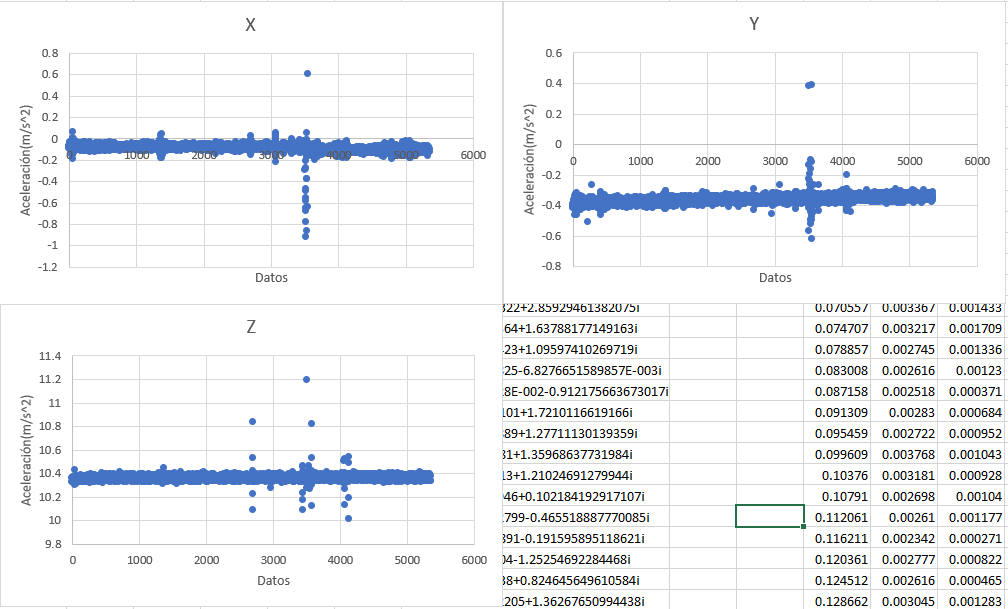
\includegraphics[width=0.6\textwidth]{reposoraw.png}
    \caption{Datos representados reposo.}
    \label{fig:reposoraw}
\end{figure}

Como se puede observar en la figura \ref{fig:reposoraw}, no hay apenas movimiento, ni variaciones, esta todos los datos bastante estables salvo algún pequeño movimiento.

\begin{figure}[h]
    \centering
    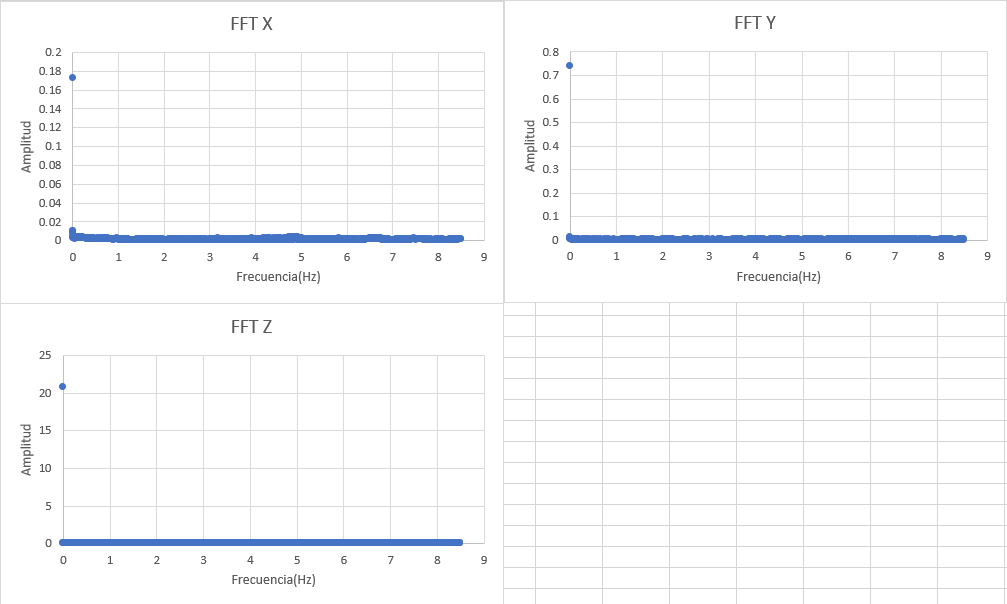
\includegraphics[width=0.6\textwidth]{reposofft.png}
    \caption{Transformada de Fourier de los datos reposo.}
    \label{fig:reposofft}
\end{figure}

La figura \ref{fig:reposofft} se representa la transformada de Fourier en la que solo están representados los datos hasta el 8.5 ya que la frecuencia es 17Hz, por lo que por la gráfica es simétrica respecto al 8.5, además del teorema de Nyquist-Shannon, que nos dice que la máxima precisión para una muestra con N datos por segundo es como mucho N/2. La transformada de Fourier no ofrece mucha información.
\subsubsection{Andando}

Ahora los datos andando, primero en bruto, y luego las transformadas de Fourier de cada variable,
\begin{figure}[h]
    \centering
    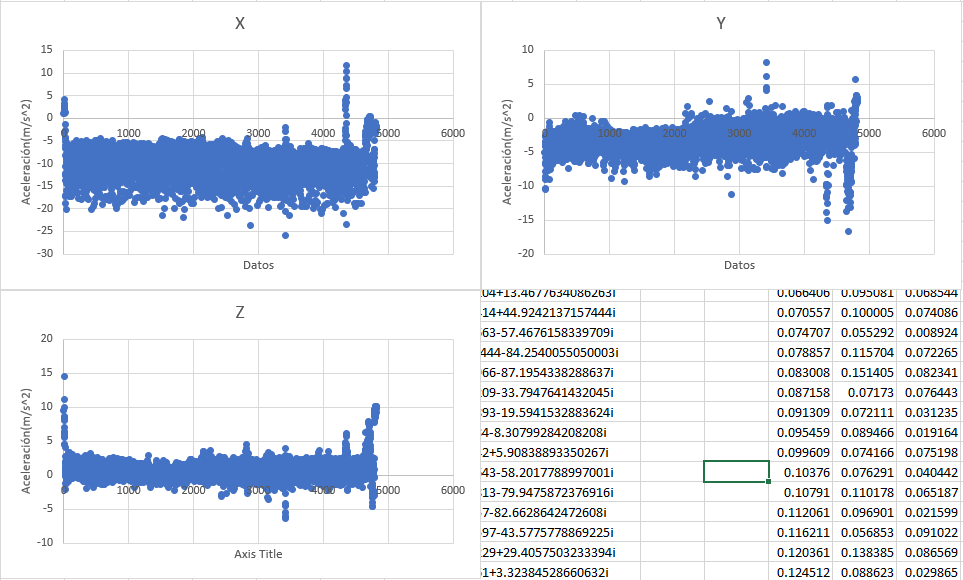
\includegraphics[width=0.6\textwidth]{andandoraw.png}
    \caption{Datos representados andando.}
    \label{fig:andandoraw}
\end{figure}

Como se podrá observar en la figura \ref{fig:andandoraw}, aquí ya no es claramente nignuna gráfica ni función a primera vista. Los picos y que esté tan dispersos(scattered) hacen que no se pueda sacar mucha información de ella. Lo que se puede saber es que la aceleración varia entre -5 y -20 para la X, 0 y -15 para la Y, y apenas en el eje Z, [-5:5].

\begin{figure}[h]
    \centering
    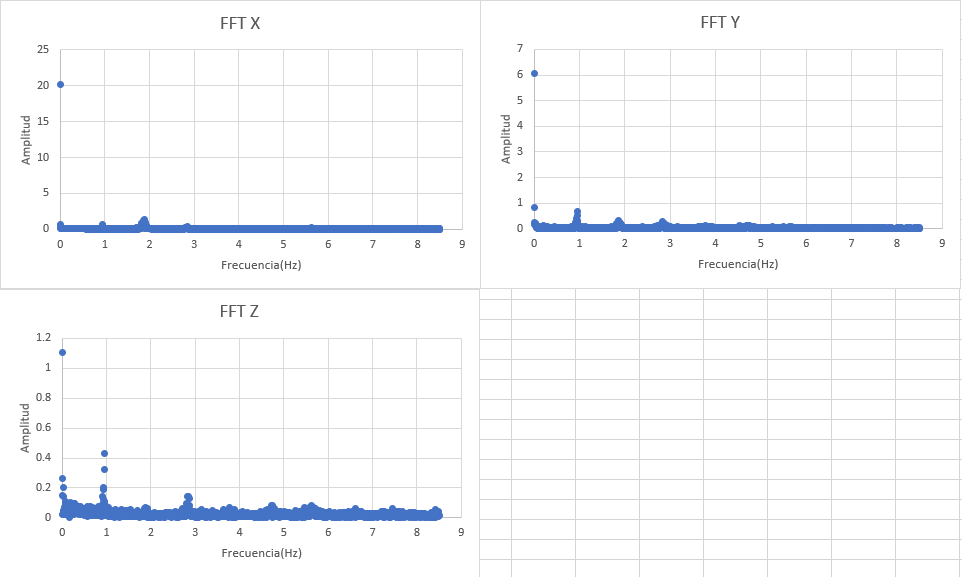
\includegraphics[width=0.7\textwidth]{andandofft.png}
    \caption{Transformada de Fourier de los datos andando.}
    \label{fig:andandofft}
\end{figure}

En la figura \ref{fig:andandofft} está la transformada de Fourier de los datos andando, y algo de información si se puede sacar, los picos nos informan de la periodicidad entorno a esas frecuencias, en este caso, el pico más destacable es el del eje Z en torno a 1 Hz.

\subsubsection{Corriendo}
\begin{figure}[h]
    \centering
    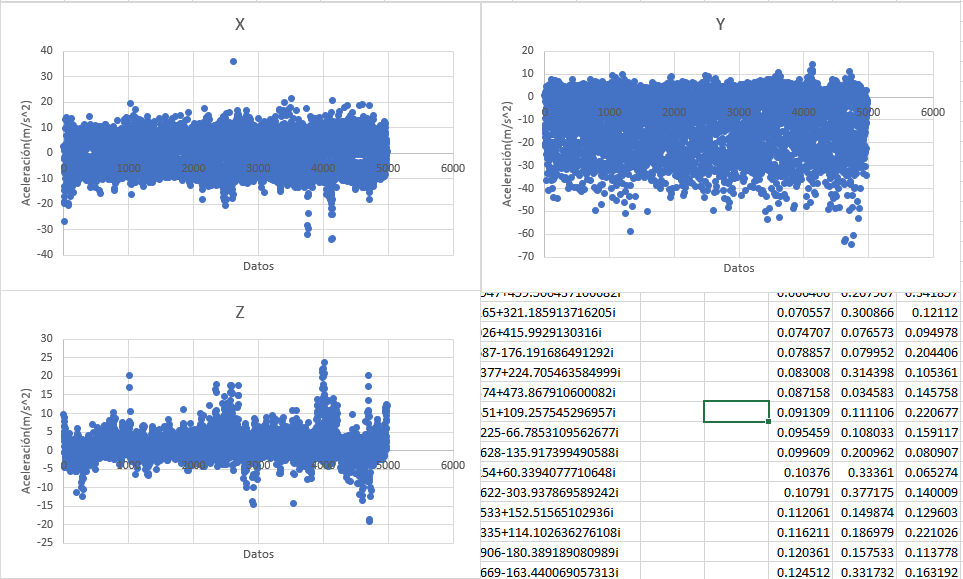
\includegraphics[width=0.6\textwidth]{corriendoraw.png}
    \caption{Datos representados corriendo.}
    \label{fig:corriendoraw}
\end{figure}

Al igual que antes, en la figura \ref{fig:corriendoraw}, los datos están desperdigados, pero podemos hacer unos rangos, [-30:10] en el X, [-40, 20] para el Y y bastante menos para el Z, [-5:20] salvando picos.
\begin{figure}[h]
    \centering
    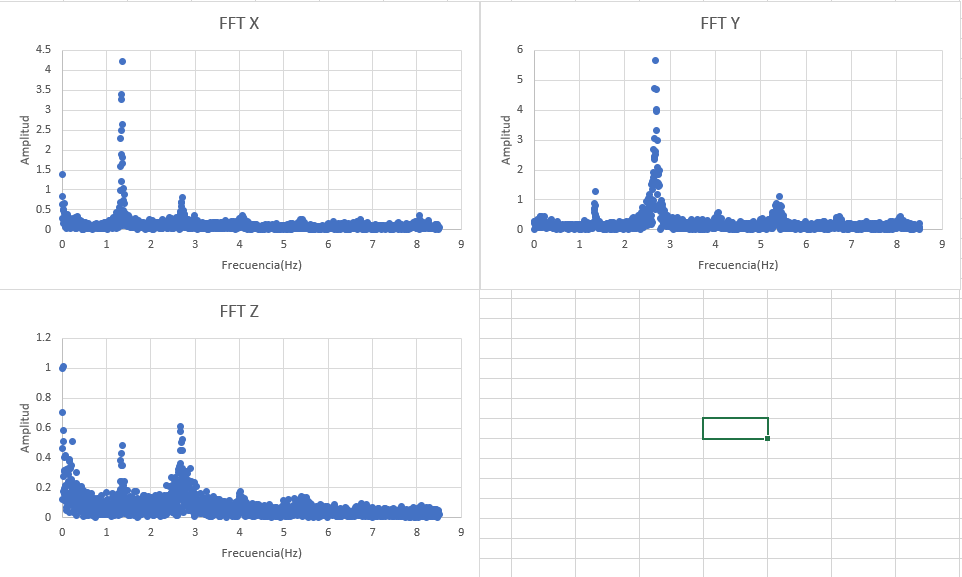
\includegraphics[width=0.6\textwidth]{corriendofft.png}
    \caption{Transformada de Fourier de los datos corriendo.}
    \label{fig:corriendofft}
\end{figure}

Ahora, como se observa en la figura \ref{fig:corriendofft}, la transformada si tiene picos más claros en todos los ejes, en torno al 1.35 en el eje X, el 2.7, y el Z en ambos, al igual que hay picos más pequeños. Lo curioso es que no tienen el mismo periodo los distintos ejes.

\subsubsection{Cayendo}

Finalmente los datos cayendo,
\begin{figure}[h]
    \centering
    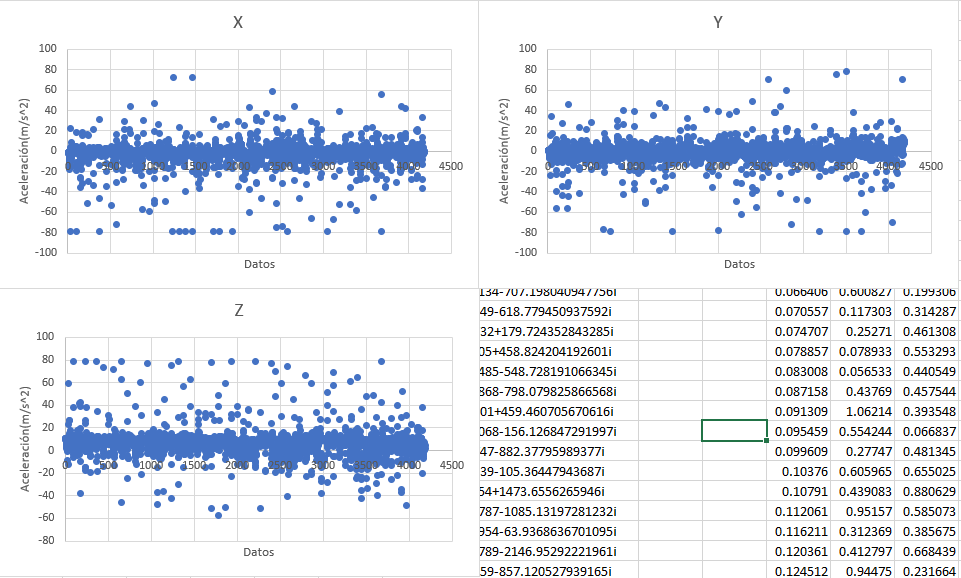
\includegraphics[width=0.6\textwidth]{cayendoraw.png}
    \caption{Datos representados cayendo.}
    \label{fig:cayendoraw}
\end{figure}
vemos ahora en la figura \ref{fig:cayendoraw} grandes picos en todas direcciones, lo que implica que el movimiento ha sido brusco. También en valores absolutos, son datos más grandes que en las gráficas anteriores, donde los datos se movían en rangos de [-20,20] y aquí se observan datos de hasta 100.

\begin{figure}[h]
    \centering
    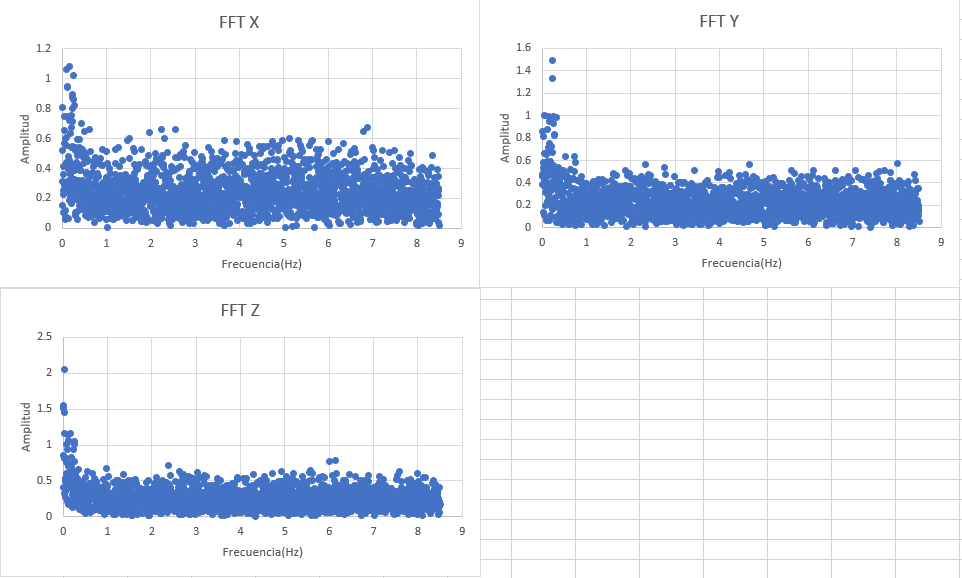
\includegraphics[width=0.6\textwidth]{cayendofft.png}
    \caption{Transformada de Fourier de los datos cayendo.}
    \label{fig:cayendofft}
\end{figure}

La transformada de Fourier, en la figura \ref{fig:cayendofft}, tampoco sirve para mucho, ya que al no haber picos, no hay una periodicidad.

\subsubsection{Comentarios de los datos}

Como se puede ver en las gráficas, en algunos casos hay elementos identificativos de que tipo de movimiento es. Los problemas de una aproximación algorítmica son varios, para empezar, hay que hacer la transformada de Fourier rápida, en tiempo real diecisiete veces por segundo para tres variables y luego ir haciendo el algoritmo que separe los tipos de movimientos. Android es un lenguaje basado en java, y las operaciones matemáticas no son especialmente eficiente en él. Esto tendría un impacto en la batería notable, y el objetivo es que consuma lo mínimo posible. Además, en el caso en el que se añadiera un nuevo movimiento implicaría unas nuevas reglas de selección del tipo de movimiento que no entre en conflicto con las existentes. Todas estos problemas hacen que una aproximación algorítmica al problema es compleja y poco eficiente en su ampliación y mantenimiento. Se puede ver un resumen de los rangos en el cuadro \ref{table1}.

\begin{center}
\begin{table}
\caption{Metodología toma de datos}
\begin{center}
\begin{tabular}{| c | c | c | c |}
\hline
 & Rango X & Rango Y & Rango Z \\
\hline
Reposo & 0 & 0 & 0\\
\hline
Andando & [-20:-5] & [-15:0] & [-5:5] \\
\hline
Corriendo & [-30:10] & [-40:20] & [-5:20] \\
\hline
Cayendo & [-100:100] & [-100:100] & [-40:80] \\
\hline
\end{tabular}
\end{center}
\label{table1}
\end{table}
\end{center}


Aunque los rangos pudieran ser identificativos, que no lo son, porque si hay un dato en 0, no se puede identificar que tipo de movimiento es, solo en los extremos únicos se puede saber exactamente el movimiento. Con esto se quiere decir, si sale -100 se puede saber perfectamente que es una caída, pero si saliera por ejemplo -40 en Y, no se puede asegurar que sea una caída o esté corriendo el usuario.

Si nos fijamos en las transformadas de Fourier, al haber varios picos,  se podría ir uno fijando, pero solo serviría para distinguir entre andando, corriendo y las otras dos, pues no tienen picos ni ningún tipo de periodicidad los datos de reposo o cayendo. 

Todo esto, junto a que el funcionamiento adecuado tampoco está asegurado de esta forma, hace que se opte por una vía distinta. Se entrenará una inteligencia artificial que se fije en estos patrones. Algunas ventajas son evidentes, la principal, la del código. La inteligencia artificial está programada y lista para ser usada en herramientas preparadas para ello. El uso es sencillo y directo.

Pero no es algo descabellado, pues en la bibliografía\cite{s150818901} se opta a menudo por esta opción.


\newpage

\newpage
\subsection{Programación}

Para extraer los datos, se ha usado las herramientas de Android. Esto simplifica mucho el trabajo ya que no hay que programar una interfaz completa de comunicación, vale con la incluida en Android. Esta es la \textit{Data Layer}. Es una capa de datos que se sincroniza entre todas las instancias del programa. Esto quiere decir que si la aplicación desde el módulo del smartwatch manda un dato a esta capa, la aplicación desde el smartphone tiene acceso a esos datos. Así, la comunicación es mucho más sencilla. En la figura \ref{fig:datalayer} se puede ver un pequeño esquema de esto.

\begin{figure}[h]
    \centering
    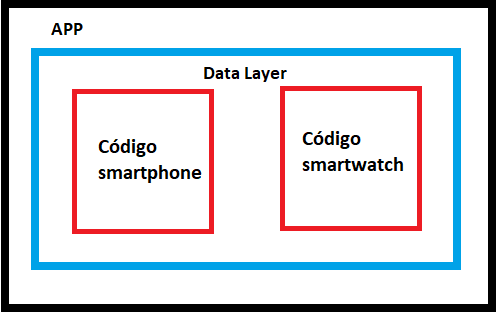
\includegraphics[width=1\textwidth]{esquemacodigo.png}
    \caption{Esquema funcionamiento de la capa de datos.}
    \label{fig:datalayer}
\end{figure}


Hay que programar el acceso a la data layer para escribir y para leer. Para ello, primero tenemos que encontrar los nodos conectados. Cada instancia de la aplicación en cada dispositivo es un nodo, en nuestro caso hay dos nodos, el del smartwatch y el del smartphone. La forma más sencilla es crear un servicio en cada nodo que se encarga automáticamente de recibir y mandar mensajes. Así, con un pequeño fragmento de código se está comprobando constantemente si hay datos nuevos y si están en el sitio que nos interesa. Hay que definir un camino(ruta) donde van a estar los datos, en el código se llama \textit{message\_path}. Si está en el lugar adecuado, entonces ese mensaje se manda a la actividad principal y se muestra en pantalla.


\begin{lstlisting}
public class ListenerService extends WearableListenerService {
    String TAG = "mobile Listener";
    @Override
    public void onMessageReceived(MessageEvent messageEvent) {

    if (messageEvent.getPath().equals("/message_path")) {
       final String message = new String(messageEvent.getData());
       Log.v(TAG, "Message path received on phone is: "
          + messageEvent.getPath());
       Log.v(TAG, "Message received on phone is: "
          + message);

       // Broadcast message to MainActivity for display
       Intent messageIntent = new Intent();
       messageIntent.setAction(Intent.ACTION_SEND);
       messageIntent.putExtra("message", message);
       LocalBroadcastManager.getInstance(this).sendBroadcast(messageIntent);
    }
    else {
        super.onMessageReceived(messageEvent);
    }
}

}

\end{lstlisting}


Aquí tenemos el código del servicio del fragmento del smartphone, que está comprobando constantemente los datos recibidos. Para buscar los nodos, usamos las herramientas que nos ofrece android

\begin{lstlisting}

public void run() {
	//first get all the nodes, ie connected wearable devices.
    Task<List<Node>> nodeListTask =
    	Wearable.getNodeClient(getApplicationContext())
                .getConnectedNodes();
        try {
        // Block on a task and get the result synchronously 
        (because this is on a background
        // thread).
        	List<Node> nodes = Tasks.await(nodeListTask);

      	    //Now send the message to each device.
            for (Node node : nodes) {
            	Task<Integer> sendMessageTask =
                	Wearable.getMessageClient
                    (MainActivity.this)
                    .sendMessage(node.getId(), path, 			                            					message.getBytes());

                try {
                	// Block on a task and get the result 	
                	synchronously 
                	(because this is on a background
                    // thread).
                    Integer result = Tasks.await(sendMessageTask);
                    sendmessage("SendThread: message send to "
                     + node.getDisplayName());
                    Log.v(TAG, "SendThread: message send to " + 
                    node.getDisplayName());

                } catch (ExecutionException exception) {
                	sendmessage("SendThread: message failed to"
                	+ node.getDisplayName());
                    Log.e(TAG, "Send Task failed: " + exception);

                } catch (InterruptedException exception) {
                    Log.e(TAG, "Send Interrupt occurred: "
                    + exception);
               }
         }
    } catch (ExecutionException exception) {
    	sendmessage("Node Task failed: " + exception);
        Log.e(TAG, "Node Task failed: " + exception);
    } catch (InterruptedException exception) {
        Log.e(TAG, "Node Interrupt occurred: " + exception);
}
}
\end{lstlisting}

Con estos dos fragmentos de código está la comunicación entre dispositivos activa. Evidentemente, la aplicación en la parte del smartwatch lleva estos mismos dos fragmentos de código también.

\newpage
\section{Resultados}

Los resultados se explican en una imagen, que es el resultado del entrenamiento de la red neuronal. Esta imagen es la matriz de confusión, que muestra como de eficaz ha sido la red en identificar los datos tras el entrenamiento.


\begin{figure}[h]
    \centering
    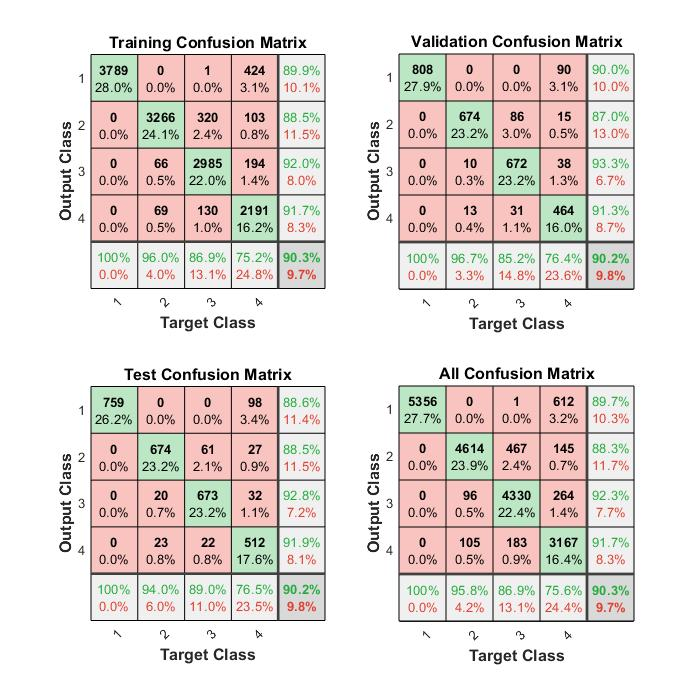
\includegraphics[width=1\textwidth]{confussionplaceholder.jpg}
    \caption{Matriz de confusión de los resultados.}
    \label{fig:mesh2}
\end{figure}

Hay cuatro matrices de confusión, una para el entrenamiento, otra para la validación, otra para la comprobación de la red y finalmente una global. Se han usado el 70\% de los datos para entrenar la red, 15\% para comprobar y 15\% para testear. Esto nos presenta unos resultados interesantes, con un acierto global del 91.1\%.

La matriz de confusión representa los datos correctos en la columna principal, es decir, los datos que son andar y la red los reconoce como andar por ejemplo. Las clases de salida son: Reposo, andando, corriendo y caídas, por ese orden. Los datos en rojo de las columnas representan los datos que son de la clase X pero la red lo detecta como Y, y las filas representan todos los datos que la red ha detectado como clase X.

De la matriz de confusión se pueden extraer muchos datos, por ejemplo, los datos de reposo apenas son confundidos, son detectados perfectamente por la red. Sin embargo, entre el resto de datos si hay más fallos. Por ejemplo, los datos de corriendo se confunden a menudo con los de andando,pero no tanto al revés, los de andar no se confunden mucho con correr. Para ello, ver en los datos totales, en el dato (2,3), que indica los datos de correr que se han detectado como andar pero son correr, es mucho mayor que los datos de (3,2), que son los datos de andar que se han detectado como correr.

Sin embargo, las mayores imprecisiones se encuentran en la columna 4. Muchos datos son confundidos con andar. Esto se debe a la metodología de toma de datos de las caídas. Al caer, se han tomado los datos hasta que el usuario queda en reposo absoluto, creando a veces momentos en los que el sistema estará en reposo, o a una velocidad mucho menor ya que en una caída, por lo que se han confundido esos momentos de la caída con reposo sobretodo, y en menor medida con andar y correr.


\newpage
\section{Conclusiones}

Teniendo en cuenta las limitaciones que nos impone Android, y al no poder tomar simultáneamente los datos del acelerómetro y del giroscopio, no funciona mal. Un 90.3\% de acierto global está bastante bien y muestra la potencia de las redes neuronales y de la inteligencia artificial.

Una lista de puntos sería:

\begin{enumerate}
\item[1.] Ha sido interesante adentrarse en el mundo de la inteligencia artificial, pues así se da uno cuenta del gran campo que hay de investigación. Además, es el momento adecuado, ya existe la potencia de computación para resolver verdaderos problemas. Se ha hecho una introducción al campo muy interesante y además muy legible, fácil de seguir y comprender.

\item[2.] El internet de las cosas sigue adelante aunque últimamente el termino este de capa caída. La potencia de los dispositivos aumenta y cada vez tienen más utilidad. En este caso se ha usado un dispositivo de uso general para algo muy concreto y que podría tener utilidad para muchas personas.

\item[3.] El potencial para el cambio de la vida de personas ancianas y/o en riesgo es alto. Con una inversión mayor se podría crear una aplicación más precisa que ayudaría a millones de personas, y además no es algo caro, ya que los smartwatch son asequibles y son cómodos de llevar. Además, muchas personas mayores están acostumbradas a llevar un reloj, así que el tiempo de adaptación sería corto.

\item[4.] El principal problema de los smartwatches sigue siendo, no su potencia, sino su batería. La mayor mejora que podrían obtener este tipo de dispositivos sería en ese campo. Hay otras opciones, como por ejemplo usar una pantalla de bajo consumo que no sea LCD. De esta forma, se podrían obtener dispositivos de batería de gran duración. Como se observó en la sección de antecedentes, la conexión a internet y el LCD hacen bastante proporción del gasto. Con un dispositivo con tecnología e-ink se podría reducir muchísimo el gasto.

\item[5.] Como nota personal, ha sido interesante adentrarse en el mundo de la programación y tratamiento de señales a un nivel más allá del necesario para superar la carrera. De esta forma, he aprendido y ampliado mis conocimientos en el campo, y además lo he disfrutado.
\end{enumerate}

Como posibles ampliaciones de este trabajo, se proponen varias cosas. La primera sería abandonar la red neuronal en MatLab y pasar a otro tipo de software que permita la importación de la red neuronal a Android, de forma que la aplicación pueda ir clasificando en tiempo real. Para ello habría que usar por ejemplo TensorFlow. Este programa permite guardar la red entrenada en un tipo de archivo que se puede implementar en aplicaciones Android de forma nativa. No es su única ventaja, otra es que es software libre, al contrario que MatLab, con lo que se conseguiría un trabajo desarrollado totalmente en software libre.

Otra posible ampliación sería tomar más datos simultáneamente, por ejemplo acelerómetro y giroscopio a la vez. No es posible en WearOS actualmente tomarlo a la vez. Se puede tomar salteado pero no se sabe si manda un dato de acelerómetro, uno de giroscopio y así sucesivamente o te manda diez datos seguidos del acelerómetro y luego otros veintiocho del giroscopio, lo cual hace que no sea viable en WearOS.




\newpage
\nocite{s150818901}
\nocite{Goodfellow-et-al-2016}
\nocite{wasserman}
\bibliographystyle{plain}
\bibliography{mybib}
\end{document}


